 \documentclass{article}

%------------------------- packages -------------------------%
\PassOptionsToPackage{obeyspaces,spaces}{url}
\usepackage[T1]{fontenc}
\usepackage[utf8]{vietnam}
\usepackage[unicode,hidelinks]{hyperref}    % for reference
\usepackage{geometry}   % for layout
\usepackage{amsmath}    % for math
\usepackage{amssymb}    % for math symbol
\usepackage{xcolor}     % for color
% for figure
\usepackage{graphicx}
\usepackage{caption}
\usepackage{subcaption}
\usepackage{tikz}
\usetikzlibrary{arrows.meta,positioning,calc,fit}
% for code
\usepackage{minted}
% for table
\usepackage{float}
\usepackage{paracol}
\usepackage{array}
\usepackage{multirow}
\usepackage{multicol}
% for header & footer
\usepackage{fancyhdr}
\usepackage{lastpage}
\usepackage{longtable}
\usepackage{enumitem}
\usepackage{array}
\usepackage{booktabs}
\usepackage{graphicx}
\usepackage{adjustbox}
%------------------------- set up -------------------------%
% renewed names
\AtBeginDocument{\renewcommand*\contentsname{Mục lục}}
\AtBeginDocument{\renewcommand*\refname{Tham khảo}}
\newcommand{\tab}{\hspace*{1cm}}
% figure
\graphicspath{{./img/}}              % path to image
\captionsetup[figure]{labelfont={small,bf,it},textfont={small,it}}
\captionsetup[table]{labelfont={small,bf},textfont={small}}
% paragraph
\setlength{\parindent}{0pt}
\setlength{\parskip}{12pt}
\setlength{\parskip}{6pt}               % disables indentation
\renewcommand{\baselinestretch}{1.5}    % line spacing
\setlength{\tabcolsep}{8pt}
\setlength{\emergencystretch}{3em}
% color
\definecolor{codegreen}{rgb}{0,0.6,0}
\definecolor{codegray}{rgb}{0.5,0.5,0.5}
\definecolor{codepurple}{rgb}{0.58,0,0.82}
% code
\def\code#1{\texttt{#1}}    % font
\newcommand{\ident}[1]{\path{#1}}   % identifier: verbatim, breakable after _ / . (not in captions/titles)
\newcommand{\tablefont}{\small\linespread{1.1}\selectfont}
\usemintedstyle{vs}         % minted theme
\setminted{
    autogobble,             % remove all common leading whitespace
    baselinestretch=1.0,
    bgcolor=gray!5!white,
    breaklines,
    %linenos,               % enables line numbers
    fontsize=\footnotesize
}
\hypersetup{
    colorlinks = true,
    urlcolor = blue,
    linkcolor = black,
}

%------------------------- layout & margin -------------------------%
\geometry{
    a4paper,        % redundant if already in \documentclass
    left=20.32mm,
    right=20.32mm,
    top=25.40mm,
    bottom=25.40mm,
    heightrounded,  % better use it
}

%------------------------- header & footer -------------------------%
\renewcommand{\headrulewidth}{0.5pt}
\renewcommand{\footrulewidth}{0.5pt}
\setlength{\headheight}{24.5pt}
\pagestyle{fancy}

\fancyhead{}    % clear all header fields
\fancyhead[L]{
    \begin{tabular}{ll}
        \begin{picture}(10,10)
            \put(0,-7){
\includegraphics[width=8mm]{img/hcmut.png}}
        \end{picture}&
    	\begin{tabular}{l}
    	    {\ttfamily Trường Đại học Bách Khoa Tp. Hồ Chí Minh} \\
    	    {\ttfamily Khoa Khoa học và Kỹ thuật Máy tính} \\
    	\end{tabular}
    \end{tabular}
}

\fancyfoot{}    % clear all footer fields
\fancyfoot[R]{\footnotesize {\ttfamily Trang {\thepage}/\pageref{LastPage}}}
% might change to \scriptsize

%------------------------- body -------------------------%
\begin{document}

%-------------------- cover --------------------%
\begin{titlepage}
\begin{center}
     \large ĐẠI HỌC QUỐC GIA THÀNH PHỐ HỒ CHÍ MINH\\
    TRƯỜNG ĐẠI HỌC BÁCH KHOA\\
    KHOA KHOA HỌC VÀ KỸ THUẬT MÁY TÍNH
\end{center}

\vspace{1.0cm}

\begin{figure}[!ht]
    \centering 
\includegraphics[width=5cm]{img/hcmut.png}
\end{figure}

\vspace{1.0cm}

\begin{table}[H]
    \centering
    \begin{tabular}{c}
    {\bf \Large Báo cáo kỹ thuật}    \\
    \\
    \hline  \\
    {\bf \large TransitPulse MBTA} \\
    {\large Giám sát xe buýt thời gian thực và cảnh báo trễ dự kiến} \\
    {\large với Kafka, Spark Structured Streaming và Cassandra} \\
    \\
    \hline
    \end{tabular}
\end{table}

\vspace{1.0cm}

\begin{table}[H]
\centering
\begin{tabular}{lrll}
& Môn học:      & Data Engineering          &         \\
& Giảng viên:   & \textbf{PGS.TS VÕ THỊ NGỌC CHÂU} &         \\
& Thành viên:   & Nguyễn Quang Minh         & 2570784 \\
&               & Trần Mậu Thật             & 2670373 \\
&               & Trần Trung Anh            & 2670252 \\
&               & Nguyễn Quỳnh Trang        & 2670382 \\
\end{tabular}
\end{table}

\vspace{1.0cm}

\begin{center}
    \footnotesize Thành phố Hồ Chí Minh, tháng 10 năm 2026
\end{center}
\end{titlepage}

\newpage
%-------------------- mission --------------------%

\newpage
%-------------------- contents --------------------%
\tableofcontents
\section{Giới thiệu}

\subsection{Bối cảnh}

Để theo dõi hoạt động của xe buýt, hệ thống cần kết hợp lịch trình với dữ liệu vận hành thực tế. Lịch trình tĩnh theo chuẩn GTFS Schedule \cite{gtfs_static} cung cấp thông tin về tuyến, trạm, chuyến, giờ chạy và hình dạng tuyến đường. Dữ liệu theo chuẩn GTFS Realtime \cite{gtfs_rt} bổ sung ba luồng cập nhật, gọi là \textit{feed}: vị trí xe (Vehicle Positions), dự báo giờ đến và rời trạm (Trip Updates), cùng cảnh báo dịch vụ (Service Alerts). Massachusetts Bay Transportation Authority (MBTA), đơn vị vận hành giao thông công cộng tại khu vực Boston, công bố hai loại dữ liệu này dưới dạng tệp ZIP và JSON để người dùng có thể truy cập công khai \cite{mbta_gtfs}.

Dữ liệu thời gian thực được cập nhật liên tục nhưng có thể thiếu trường, đến trễ, ngừng cập nhật hoặc lặp lại nội dung đã nhận. Vì vậy, chỉ hiển thị phản hồi mới nhất từ nguồn là chưa đủ. Hệ thống còn cần làm rõ:
\begin{itemize}
    \item Vị trí xe được ghi nhận lúc nào và còn đủ mới để sử dụng hay không?
    \item Giờ đến trạm là dự báo từ dữ liệu thời gian thực hay chỉ là giờ theo lịch trình?
    \item Kết quả đang hiển thị đã được xử lý đầy đủ hay còn thiếu do quá trình ghi dữ liệu bị gián đoạn?
\end{itemize}

Từ các yêu cầu trên, nhóm xây dựng TransitPulse MBTA trong khuôn khổ đồ án môn Data Engineering. Hệ thống sử dụng Apache Cassandra \cite{cassandra} để lưu trữ và quản lý dữ liệu, Apache Spark Structured Streaming \cite{spark,structured_streaming} để xử lý dữ liệu luồng, Apache Kafka để chuyển các sự kiện giữa các thành phần và FastAPI để cung cấp kết quả cho giao diện người dùng.

\subsection{Mục tiêu}

Mục tiêu của dự án là xây dựng một quy trình hoàn chỉnh: thu thập dữ liệu xe buýt MBTA, xử lý qua chuỗi \textbf{Kafka $\rightarrow$ Spark Structured Streaming $\rightarrow$ Cassandra}, sau đó cung cấp kết quả qua FastAPI cho giao diện React, bảng theo dõi Streamlit và notebook trên Google Colab. Bên cạnh việc hiển thị kết quả, hệ thống cần đáp ứng các yêu cầu về độ tin cậy của dữ liệu:

\begin{itemize}
    \item \textbf{Quản lý phiên bản}: mỗi kết quả được gắn với một lần chạy (\textit{run}), một bản chụp dữ liệu nguồn (\textit{snapshot}) và một phiên bản dữ liệu phục vụ truy vấn (\textit{generation}). Khi đã tạo, nội dung của generation không thay đổi.
    \item \textbf{Phân biệt các mốc thời gian}: thời điểm ghi nhận vị trí xe, thời điểm tạo feed và thời điểm hệ thống xử lý được lưu riêng để tránh nhầm lẫn khi đánh giá độ mới của dữ liệu.
    \item \textbf{Kiểm soát chất lượng}: các bản ghi bị loại, cách ly hoặc xác định là trùng lặp đều có mã lý do và tham chiếu đến dữ liệu gốc.
    \item \textbf{Phục hồi khi có lỗi}: quá trình xử lý lại cần giữ nguyên kết quả logic, tránh hiển thị dữ liệu ghi dở, đếm trùng KPI hoặc thay thế trạng thái mới bằng dữ liệu cũ.
    \item \textbf{Truy vết nguồn gốc}: từ kết quả trên API có thể xác định Kafka offset, tệp dữ liệu gốc và giá trị kiểm tra toàn vẹn (checksum) của lần thu thập tương ứng.
\end{itemize}

\subsection{Người dùng và câu hỏi nghiệp vụ}

Bảng~\ref{tab:users} liệt kê bốn nhóm người dùng và thông tin mà mỗi nhóm cần.

\begin{table}[H]
\centering
\tablefont
\caption{Người dùng mục tiêu của TransitPulse}
\label{tab:users}
\begin{tabular}{p{3.10cm}p{6.01cm}p{6.01cm}}
\toprule
\textbf{Vai trò} & \textbf{Câu hỏi cần trả lời} & \textbf{Thông tin hệ thống cung cấp} \\
\midrule
Hành khách & Xe ở đâu, khi nào tới trạm, tuyến có gián đoạn không & Bản đồ xe theo tuyến, ETA theo trạm có nhãn chất lượng, cảnh báo dịch vụ \\
Người theo dõi vận hành & Tuyến nào có dự báo chậm, bao nhiêu xe có vị trí mới & KPI ``độ trễ dự kiến'' kèm tử số, mẫu số và thời điểm tính \\
Kỹ sư dữ liệu & Nguồn còn cập nhật không, lỗi ở bước nào, có dữ liệu chờ xử lý không & Trang chất lượng và trạng thái xử lý, hàng đợi lỗi (DLQ), tham chiếu dữ liệu gốc và thông tin truy vết \\
Người đánh giá & Dữ liệu có đi qua Kafka, Spark, Cassandra và cho kết quả đúng không & Kiểm thử golden smoke, báo cáo kiểm thử, kịch bản lỗi và kết quả đo hiệu năng \\
\bottomrule
\end{tabular}
\end{table}

\subsection{Phạm vi}

Phiên chạy thử đã thực hiện trên \textbf{10 tuyến xe buýt} của MBTA (\ident{route_type=3}): \ident{1}, \ident{15}, \ident{22}, \ident{23}, \ident{28}, \ident{32}, \ident{39}, \ident{57}, \ident{66} và \ident{77}. Danh sách tuyến được đối chiếu với GTFS tại thời điểm chạy. Mỗi lần chạy sử dụng một phiên bản GTFS cố định. Hệ thống hỗ trợ ba chế độ, cùng đi qua một quy trình xử lý:
\begin{itemize}
    \item \textbf{live}: thu thập trực tiếp ba feed MBTA theo chu kỳ 30 giây;
    \item \textbf{replay}: phát lại dữ liệu đã ghi ở tốc độ 1x, 10x hoặc 50x, có thể tạm dừng và tiếp tục;
    \item \textbf{synthetic}: phát dữ liệu mô phỏng được sinh theo quy tắc tất định. Dữ liệu này mang nhãn \ident{source_type=synthetic} và không được hiển thị như dữ liệu xe MBTA thực tế.
\end{itemize}

Dự án chưa xây dựng mô hình dự báo giờ đến trạm (ETA) riêng, chưa đánh giá độ chính xác ETA do thiếu dữ liệu thực tế làm đối chứng (ground truth), và chưa thực hiện tối ưu hành trình hay đếm hành khách. Hạ tầng có tính sẵn sàng cao và triển khai trên nhiều vùng cũng nằm ngoài phạm vi đồ án. ETA hiển thị được lấy từ dự báo của MBTA. Trong báo cáo, ``độ trễ dự kiến'' được hiểu là chênh lệch giữa giờ dự báo và giờ theo lịch GTFS; chỉ số này không thể hiện độ trễ thực tế hoặc chỉ số đúng giờ chính thức của MBTA.

\subsection{Đóng góp chính}

\begin{enumerate}
    \item Xây dựng quy trình xử lý từ đầu đến cuối trên máy ảo Google Colab. Các thành phần được chạy trực tiếp bằng tệp nhị phân, không cần Docker hay quyền sudo, gồm Kafka 4.2.2 (KRaft), Cassandra 5.0.9, Spark 3.5.7, bộ thu thập dữ liệu, FastAPI và ba loại giao diện.
    \item Thiết kế cơ chế công bố dữ liệu dựa trên generation bất biến. Bản mô tả generation (manifest) ghi nhận trạng thái \ident{BUILDING}/\ident{READY}, còn con trỏ \ident{feed_current} được cập nhật bằng compare-and-set, sử dụng lightweight transaction của Cassandra. Trong điều kiện không có giao dịch chung giữa Kafka, hệ thống tệp và Cassandra, cách làm này hỗ trợ giao nhận ít nhất một lần (at-least-once), đồng thời cho phép ghi và công bố lại mà không thay đổi kết quả logic (idempotent).
    \item Xây dựng các mã định danh tất định (\ident{snapshot_id}, \ident{observation_id}, \ident{prediction_id}, \ldots), cho kết quả thống nhất trên Python và Spark. Nhờ đó, việc thử lại hoặc phát lại dữ liệu không tạo thêm bản ghi trùng.
    \item Phân biệt đồng hồ nguồn, đồng hồ hệ thống và đồng hồ nghiệp vụ; xử lý giờ GTFS vượt 24:00 và ngày chuyển đổi giờ mùa hè (DST).
    \item Tính KPI độ trễ dự kiến theo quy tắc chọn một trạm mục tiêu (\textit{target stop}) cho mỗi chuyến. Kết quả đi kèm tử số, mẫu số, các lý do loại trừ và thời điểm tính để người đọc có thể kiểm tra.
    \item Xây dựng nhiều lớp kiểm chứng: bộ dữ liệu mẫu có kết quả kỳ vọng được xác định thủ công (golden fixture), bộ tính kết quả đối chứng độc lập (oracle) chỉ dùng thư viện chuẩn Python, các kịch bản chủ động gây lỗi (fault injection) và bộ công cụ đo hiệu năng (benchmark) chỉ ghi nhận số đo thực tế.
\end{enumerate}

\subsection{Cấu trúc báo cáo}

Phần~\ref{sec:problem} trình bày nguồn dữ liệu, các khó khăn kỹ thuật, yêu cầu hệ thống và cách tính các chỉ số. Phần~\ref{sec:design} mô tả kiến trúc cùng thiết kế của từng thành phần, từ thu thập, chuyển và xử lý dữ liệu đến lưu trữ trên Cassandra, công bố kết quả và vận hành. Phần~\ref{sec:experiments} trình bày phương pháp kiểm chứng, kết quả chạy thực tế, giao diện và các phép đo hiệu năng trên Google Colab. Cuối cùng, Phần~\ref{sec:conclusion} tổng kết kết quả, nêu hạn chế và đề xuất hướng phát triển. Mã nguồn của dự án được công bố tại \cite{repo}.

\section{Bài toán và yêu cầu}
\label{sec:problem}

\subsection{Nguồn dữ liệu}

Dự án sử dụng bốn nguồn dữ liệu công khai của MBTA, được liệt kê trong Bảng~\ref{tab:sources}. Các nguồn này cung cấp cả lịch trình và thông tin vận hành theo thời gian thực. Hệ thống không phụ thuộc vào MBTA V3 API hay nguồn dữ liệu khác; khi xảy ra lỗi mạng, dữ liệu MBTA cũng không được thay bằng dữ liệu từ nguồn khác.

\begin{table}[H]
\centering
\tablefont
\caption{Bốn nguồn dữ liệu MBTA được sử dụng}
\label{tab:sources}
\begin{tabular}{p{2.91cm}p{6.21cm}p{6.01cm}}
\toprule
\textbf{Nguồn} & \textbf{URL} & \textbf{Vai trò} \\
\midrule
GTFS Static & \url{https://cdn.mbta.com/MBTA_GTFS.zip} & Tuyến, trạm, chuyến, lịch trình, hình học tuyến và múi giờ \\
Vehicle Positions & \url{https://cdn.mbta.com/realtime/VehiclePositions.json} & Vị trí xe, thông tin nhận diện chuyến và thời điểm quan sát \\
Trip Updates & \url{https://cdn.mbta.com/realtime/TripUpdates.json} & Giờ dự báo đến/rời trạm và trường \ident{uncertainty} \\
Service Alerts & \url{https://cdn.mbta.com/realtime/Alerts.json} & Cảnh báo dịch vụ, đối tượng áp dụng và thời hạn hiệu lực \\
\bottomrule
\end{tabular}
\end{table}

GTFS Static lưu thông tin lịch trình trong các bảng \ident{routes}, \ident{trips}, \ident{stop_times}, \ident{stops}, \ident{calendar}, \ident{calendar_dates} và \ident{shapes}. Trong khi đó, mỗi luồng dữ liệu GTFS Realtime (feed) gồm phần \ident{header} và danh sách \ident{entity}. Header chứa phiên bản, \ident{incrementality} và \ident{timestamp} của feed; nội dung entity phụ thuộc vào loại feed.

Cụ thể, Vehicle Positions cung cấp mã xe, tọa độ, \ident{timestamp} của lần đo và thông tin nhận diện chuyến. Trip Updates chứa danh sách \ident{stop_time_update}, trong đó mỗi phần tử có giờ dự báo đến trạm (arrival), rời trạm (departure), hoặc cả hai, cùng trường \ident{uncertainty}. Service Alerts dùng \ident{informed_entity} để xác định đối tượng áp dụng theo tuyến, trạm, chuyến, đơn vị vận hành hoặc loại tuyến; \ident{active_period} xác định thời gian cảnh báo có hiệu lực.

Trong dữ liệu quan sát ngày 06/10/2026, feed Trip Updates của MBTA \textbf{không có trường \ident{delay}}. Vì vậy, hệ thống tính độ trễ dự kiến bằng cách lấy giờ dự báo trừ giờ lịch GTFS. Hai mốc được so sánh phải thuộc \textbf{cùng loại sự kiện}: giờ đến so với giờ đến, giờ rời so với giờ rời.

\subsection{Thách thức kỹ thuật}

\paragraph{Dữ liệu nguồn có thể thiếu hoặc không hợp lệ.} Một entity có thể thiếu \ident{vehicle.id}, có tọa độ ngoài miền hợp lệ hoặc có \ident{timestamp} ở tương lai. Thời gian cũng có thể được ghi theo mili giây thay vì giây. Ngoài ra, một chuyến có thể đi qua cùng một trạm hai lần, nên chỉ dùng \ident{stop_id} là chưa đủ để ghép dự báo với lịch trình.

\paragraph{Dữ liệu có thể được xử lý nhiều lần.} Với cơ chế giao nhận at-least-once, Kafka và checkpoint của Spark hỗ trợ tránh mất thông điệp, nhưng một thông điệp vẫn có thể được xử lý nhiều lần. Chẳng hạn, bộ thu thập (collector) có thể gửi lại dữ liệu sau khi khởi động lại, hoặc Spark có thể xử lý lại một lô nhỏ (micro-batch) sau sự cố. Một bản chụp dữ liệu tại thời điểm thu thập (snapshot) cũ cũng có thể đến sau snapshot mới. Trong các trường hợp này, kết quả logic của hệ thống cần được giữ nhất quán.

\paragraph{Không có giao dịch chung giữa các thành phần.} Trong một lần xử lý, hệ thống ghi dữ liệu vào Kafka qua DLQ, vào hệ thống tệp dưới dạng curated Parquet và vào nhiều bảng Cassandra. Ba nơi lưu trữ này không có cơ chế xác nhận ghi nguyên tử chung. Vì vậy, hệ thống cần kiểm soát thời điểm đưa một phiên bản dữ liệu (generation) vào phục vụ, tránh để API đọc dữ liệu khi quá trình ghi chưa hoàn tất.

\paragraph{Phân biệt các mốc thời gian.} Thời điểm đo vị trí xe, tạo feed, thu thập, gửi lên Kafka và hiển thị dữ liệu là các mốc khác nhau. Lịch GTFS còn cho phép giờ vượt 24:00 để biểu diễn các chuyến qua nửa đêm. Vào ngày đổi giờ mùa hè, cách cộng trực tiếp giờ lịch vào mốc nửa đêm có thể cho kết quả lệch một giờ. Khi phát lại dữ liệu (replay), thời điểm hiện tại được xác định theo đồng hồ của bản ghi lịch sử, thay vì giờ máy.

\paragraph{Thiết kế dữ liệu theo truy vấn của Cassandra.} Cassandra không hỗ trợ phép nối bảng. Truy vấn ngoài khóa phân vùng có thể cần \ident{ALLOW FILTERING} và phải quét toàn bảng. Do đó, mô hình dữ liệu được xây dựng từ nhu cầu truy vấn (query-first), để mỗi endpoint đọc theo phân vùng và giới hạn số bản ghi bằng \ident{LIMIT}.

\subsection{Yêu cầu chức năng}

Bảng~\ref{tab:fr} trình bày 12 yêu cầu chức năng cùng các thành phần đảm nhận từng yêu cầu.

\begingroup\tablefont
\begin{longtable}{p{1.16cm}p{8.73cm}p{5.24cm}}
\caption{Yêu cầu chức năng và thành phần thực hiện} \label{tab:fr} \\
\toprule
\textbf{Mã} & \textbf{Yêu cầu} & \textbf{Thành phần} \\
\midrule
\endfirsthead
\toprule
\textbf{Mã} & \textbf{Yêu cầu} & \textbf{Thành phần} \\
\midrule
\endhead
FR01 & Nhập tệp GTFS ZIP; dùng SHA-256 của tệp làm phiên bản; lưu bảng chiều Parquet và metadata bất biến & \ident{static/} \\
FR02 & Thu thập độc lập 3 feed; lưu dữ liệu gốc và metadata trước khi gửi; không tạo snapshot rỗng khi hết thời gian chờ & \ident{ingestion/collector.py}, \ident{archive.py} \\
FR03 & Gửi snapshot qua Kafka với schema, checksum và ID ổn định; lưu bền vững hàng đợi gửi (outbox) & \ident{ingestion/outbox.py}, \ident{kafka_producer.py} \\
FR04 & Dùng Spark để phân tích, kiểm tra, tách phần tử, nối với GTFS và loại trùng; gắn mã chất lượng và tham chiếu dữ liệu gốc & \ident{processing/} \\
FR05 & Lấy vị trí xe từ generation hiện tại; phân lớp fresh/stale/unknown/invalid; không cộng dồn số xe qua nhiều snapshot & \ident{processing/vehicles.py}, \ident{api/freshness.py} \\
FR06 & Cung cấp dự báo đến/rời trạm, uncertainty của MBTA và độ trễ dự kiến khi xác định được lịch & \ident{processing/predictions.py}, \ident{schedule.py} \\
FR07 & Tính KPI tuyến với tối đa một trạm mục tiêu cho mỗi chuyến trong ngày dịch vụ; công bố tử số, mẫu số, lý do loại trừ và thời điểm tính & \ident{processing/kpi.py} \\
FR08 & Xác định đối tượng và thời hạn của cảnh báo; phân biệt cảnh báo MBTA với cảnh báo chất lượng pipeline & \ident{processing/alerts.py}, API \ident{/alerts} \\
FR09 & Phân trang lịch sử xe; lưu dữ liệu đã xử lý dưới dạng curated Parquet; lập báo cáo lịch sử bằng Spark batch & \ident{processing/report_job.py} \\
FR10 & Giữ generation bất biến; API chỉ đọc READY; dữ liệu trùng, đến muộn hoặc xử lý lại không làm tăng KPI hay lùi con trỏ & \ident{processing/batch.py}, \ident{storage/pointer.py} \\
FR11 & Phát lại với đúng phiên bản dữ liệu tĩnh ở tốc độ 1x/10x/50x, có tạm dừng/tiếp tục; tách đồng hồ nguồn khỏi đồng hồ máy & \ident{replay/} \\
FR12 & Cung cấp API, dashboard, trang chất lượng; kiểm thử golden, kiểm thử lỗi và benchmark có bằng chứng & \ident{api/}, \ident{app/}, \ident{tests/}, \ident{benchmarks/} \\
\bottomrule
\end{longtable}
\endgroup

\subsection{Yêu cầu phi chức năng}

\begin{table}[H]
\centering
\tablefont
\caption{Yêu cầu phi chức năng}
\label{tab:nfr}
\begin{tabular}{p{1.37cm}p{3.34cm}p{10.42cm}}
\toprule
\textbf{Mã} & \textbf{Thuộc tính} & \textbf{Cách đáp ứng} \\
\midrule
NFR01 & Tính đúng & Bộ dữ liệu chuẩn (golden fixture) viết tay và bộ tính kết quả đối chiếu (oracle) độc lập \ident{tests/oracle/} \\
NFR02 & Phục hồi & Checkpoint của Spark, ghi đầu ra lặp lại không làm đổi kết quả (idempotent), manifest cố định và outbox bền vững \\
NFR03 & Độ trễ & Mục tiêu p95 của độ trễ đưa dữ liệu vào phục vụ (visibility latency) $<$ 10 s; cần kiểm chứng bằng benchmark \\
NFR04 & Dung lượng & Gói thông điệp (envelope) $\le$ 4 MiB, thời gian lưu topic 6 giờ, dung lượng dành cho dữ liệu gốc 2 GiB \\
NFR05 & Truy vết & Lần theo nguồn gốc dữ liệu từ API về manifest, Kafka offset và checksum của dữ liệu gốc \\
NFR06 & Tái lập & Cố định phiên bản bằng \ident{==}, dùng seed tất định và manifest môi trường chạy có checksum \\
NFR07 & Theo dõi vận hành & Log JSON có cấu trúc, chỉ số Prometheus và \ident{/pipeline/status} \\
NFR08 & Giới hạn truy vấn & Không dùng \ident{ALLOW FILTERING}; mọi truy vấn đọc có \ident{LIMIT} và phân trang bằng token \\
NFR09 & An toàn demo & Các cổng chỉ lắng nghe tại \ident{127.0.0.1}; giới hạn nguồn truy cập CORS; không công khai Kafka/Cassandra \\
NFR10 & Demo ngoại tuyến & Phát lại bản ghi và chạy dữ liệu tổng hợp (synthetic) khi không có kết nối tới MBTA \\
\bottomrule
\end{tabular}
\end{table}

\subsection{Định nghĩa và cách tính các chỉ số}
\label{sec:metrics}

Phần này trình bày cách tính và điều kiện sử dụng các chỉ số của hệ thống. Các ngưỡng được xác định theo \textbf{chính sách của dự án} (policy) và được lưu cố định trong \ident{run_metadata.policy_json} khi tạo một lần chạy (run). Đây là các quy tắc phục vụ dự án, không phải cam kết mức dịch vụ (SLA) của MBTA.

\subsubsection{Độ mới của vị trí xe}

Gọi $c$ là thời gian theo đồng hồ nghiệp vụ (application clock) tại lúc đánh giá và $t_{obs}$ là thời điểm nguồn đo vị trí xe. Tuổi của quan sát, tức khoảng thời gian đã trôi qua kể từ lần đo, được tính bằng
\begin{equation}
a = c - t_{obs}.
\end{equation}
Hệ thống dùng ngưỡng dữ liệu cũ (stale) $\theta_v = 120$ giây và cho phép lệch về tương lai tối đa $\epsilon = 5$ giây. Trạng thái vị trí của mỗi xe được xác định như sau:
\begin{equation}
\text{class}(a) =
\begin{cases}
\text{invalid} & \text{nếu vị trí không hợp lệ, hoặc } a < -\epsilon \ (\texttt{FUTURE\_TIMESTAMP}),\\
\text{unknown} & \text{nếu } t_{obs} \text{ không có } (a = \text{null}),\\
\text{fresh} & \text{nếu } -\epsilon \le a \le \theta_v \ (a<0 \text{ được gắn cờ } \texttt{CLOCK\_SKEW} \text{ và hiển thị } 0),\\
\text{stale} & \text{nếu } a > \theta_v.
\end{cases}
\end{equation}
Timestamp lớn hơn $10^{11}$ được xem là sai đơn vị, gắn mã \texttt{INVALID\_TIMESTAMP\_UNIT} và không được tự động quy đổi. Trạng thái độ mới (freshness) được API tính lại trong mỗi yêu cầu thay vì lưu cố định trong Cassandra. Nhờ đó, khi feed ngừng cập nhật, vị trí xe vẫn chuyển sang stale dù hệ thống không nhận thêm thông điệp. Hàm phân lớp trong \ident{contracts/policy.py} được trình bày dưới đây:

\begin{minted}{python}
def vehicle_freshness(*, position_valid, observation_time, application_clock, policy):
    if not position_valid:
        return FreshnessResult(FreshnessClass.INVALID, None, ())
    if observation_time is None:
        return FreshnessResult(FreshnessClass.UNKNOWN, None, ())
    age = (application_clock - observation_time).total_seconds()
    if age < -policy.future_tolerance_seconds:
        return FreshnessResult(FreshnessClass.INVALID, None, ("FUTURE_TIMESTAMP",))
    if age < 0:
        return FreshnessResult(FreshnessClass.FRESH, 0.0, ("CLOCK_SKEW",))
    if age <= policy.vehicle_stale_seconds:
        return FreshnessResult(FreshnessClass.FRESH, age, ())
    return FreshnessResult(FreshnessClass.STALE, age, ())
\end{minted}

Đối với từng feed, ngưỡng stale được tính theo thời gian đã trôi qua kể từ timestamp trong header: 120 giây cho Vehicle Positions, 90 giây cho Trip Updates và 300 giây cho Alerts. Tài liệu GTFS Realtime Best Practices khuyến nghị tuổi dữ liệu tối đa là 90 giây cho VP/TU và 10 phút cho Alerts \cite{gtfs_rt_bp}.

\subsubsection{Chuyển giờ GTFS sang UTC}

GTFS biểu diễn giờ bằng định dạng \texttt{HH:MM:SS}, tính từ mốc của ngày dịch vụ; giá trị \texttt{HH} có thể lớn hơn hoặc bằng 24. Theo chuẩn GTFS, mốc này được xác định bằng cách lấy ``trưa giờ địa phương trừ 12 giờ'' \cite{gtfs_static}. Cách xác định đó áp dụng cả trong ngày đổi giờ mùa hè:
\begin{align}
s_{gtfs} &= 3600\cdot HH + 60\cdot MM + SS, \\
t_{anchor} &= \text{UTC}\big(\text{trưa địa phương của ngày dịch vụ } D\big) - 12\,\text{h}, \\
t_{sched} &= t_{anchor} + s_{gtfs}.
\end{align}
Ví dụ, trong múi giờ \ident{America/New_York}, ngày 2026-03-08 là ngày chuyển sang EDT. Giờ GTFS \texttt{01:30:00} tương ứng với \texttt{2026-03-08T05:30:00Z}. Nếu cộng trực tiếp số giờ vào mốc nửa đêm mà không xét quy tắc trên, kết quả sẽ lệch một giờ. Trên Spark, hệ thống tính \ident{to_utc_timestamp('<date> 12:00:00', tz)} rồi trừ 43\,200 giây, đồng thời bắt buộc đặt \ident{spark.sql.session.timeZone=UTC}.

\subsubsection{Độ trễ dự kiến và phân loại uncertainty}

Với một sự kiện $e$ là đến trạm (arrival) hoặc rời trạm (departure), độ trễ dự kiến chỉ được tính khi đã xác định được lịch của lần ghé trạm tương ứng:
\begin{equation}
d_e = t^{pred}_e - t^{sched}_e,
\end{equation}
trong công thức này, $t^{sched}_e$ là giờ lịch của \textbf{cùng loại sự kiện} với giờ dự báo. Giá trị $d_e$ âm cho biết xe được dự báo đến hoặc rời sớm hơn lịch. Nếu ngày dịch vụ còn mơ hồ (ambiguous) hoặc chưa xác định được (unresolved), hệ thống đặt $d_e = \text{null}$ và loại sự kiện khỏi KPI. Khi đó, giờ dự báo do nguồn cung cấp vẫn được hiển thị.

Trường \ident{uncertainty} trong dữ liệu xe buýt MBTA có cách diễn giải riêng \cite{mbta_gtfs}. Bộ chuyển đổi \ident{mbta_bus_uncertainty_v1} phân loại giá trị $u$ theo các trường hợp sau:
\begin{equation}
\text{uc}(u) =
\begin{cases}
\text{unknown\_uncertainty} & u \text{ không có (vẫn eligible, đếm riêng)},\\
\text{realtime} & 0 \le u < 300,\\
\text{schedule\_only} & u = 300,\\
\text{degraded} & u = 301,\\
\text{invalid} & u < 0 \text{ hoặc } u > 301.
\end{cases}
\end{equation}

\subsubsection{KPI độ trễ dự kiến theo tuyến}

KPI được tính theo \textit{trip instance}, tức một \ident{trip_id} trong một ngày dịch vụ, thay vì tính trên từng dự báo. Với mỗi trip instance, chính sách \ident{first_future_resolved_stop_v1} chọn tối đa một sự kiện mục tiêu (\textit{target event}). Cụ thể, hệ thống xét các sự kiện có thời gian sau \ident{metrics_as_of}, đã xác định được trạm và không mang quan hệ \ident{SKIPPED}/\ident{NO_DATA}, rồi chọn sự kiện có \ident{stop_sequence} nhỏ nhất. Tại mỗi lần ghé trạm, giờ đến được ưu tiên; nếu thiếu thì dùng giờ rời.

Sau khi chọn sự kiện mục tiêu, hệ thống chỉ đánh giá tính hợp lệ của sự kiện đó. Nếu chất lượng dự báo không đạt yêu cầu, hệ thống không chuyển sang trạm tiếp theo để thay thế.

Nếu một trip instance không đủ điều kiện tính KPI, hệ thống ghi nhận \textbf{lý do đầu tiên khớp} trong thứ tự cố định sau: \ident{CANCELED_TRIP}, \ident{ADDED_TRIP}, \ident{AMBIGUOUS_SERVICE_DATE}, \ident{UNRESOLVED_TRIP}, \ident{UNRESOLVED_STOP_SEQUENCE}, \ident{NO_TARGET_STOP}, \ident{SCHEDULE_ONLY_PREDICTION}, \ident{DEGRADED_PREDICTION}, \ident{INVALID_PREDICTION}, \ident{NO_SCHEDULED_EVENT}. Gọi $E_r$ là tập trip instance đủ điều kiện (eligible) của tuyến $r$ và $d_i$ là độ trễ tại sự kiện mục tiêu của chuyến $i$. Với ngưỡng trễ $\theta_{late} = 300$ giây, các chỉ số được tính như sau:
\begin{align}
L_r &= \{\, i \in E_r : d_i \ge \theta_{late} \,\}, \\
\text{predicted\_late\_rate}_r &=
\begin{cases}
|L_r| \,/\, |E_r| & |E_r| > 0,\\
\text{null} & |E_r| = 0,
\end{cases} \\
\text{mean\_predicted\_delay}_r &= \frac{1}{|E_r|}\sum_{i \in E_r} d_i \quad (\text{null nếu } |E_r| = 0).
\end{align}
Khi không có chuyến đủ điều kiện, mẫu số bằng 0 và tỷ lệ nhận giá trị \ident{null}. Giao diện hiển thị ``Chưa có mẫu đủ điều kiện'' thay cho 0\%, để tránh hiểu nhầm rằng tất cả các chuyến đều không trễ. Mỗi KPI được công bố kèm thời điểm \ident{metrics_as_of}, tử số, mẫu số, \ident{excluded_trip_counts} và \ident{policy_version}.

\textbf{Ví dụ với golden fixture trên tuyến synthetic R\_A.} Tại thời điểm 12:00:30Z, hệ thống xét hai chuyến. Với T1, sự kiện mục tiêu là đến S3 (\ident{stop_sequence} 3), có giờ dự báo 12:11:00Z và giờ lịch 12:05:00Z, nên $d = 360$ s. Với T2, sự kiện tại \ident{stop_sequence} 1 lúc 12:00:00Z đã qua. Vì vậy, hệ thống chọn sự kiện đến S3 (\ident{stop_sequence} 2), có giờ dự báo 12:06:00Z và giờ lịch 12:05:00Z, nên $d = 60$ s.

Cả hai chuyến đều đủ điều kiện tính KPI. Khi đó, $|E| = 2$, $|L| = 1$, tỷ lệ trễ dự kiến bằng $0{,}5$ và độ trễ dự kiến trung bình bằng $(360+60)/2 = 210$ s. Dù có nhiều dự báo đến và rời tại các trạm, mỗi chuyến vẫn chỉ đóng góp tối đa 1 vào mẫu số.

\subsubsection{Đối soát số lượng dữ liệu}

Trước khi đánh dấu một generation là READY, hệ thống đối soát số lượng dữ liệu qua các đẳng thức dưới đây. Hai vế của mỗi đẳng thức phải dùng cùng đơn vị đếm:
\begin{align*}
\text{selected\_entities} &= \text{fully\_valid} + \text{partially\_valid} + \text{rejected},\\
\text{valid\_candidate\_observations} &= \text{unique\_observations} + \text{duplicate\_observations},\\
\text{membership}_{(route)} &= \text{fresh} + \text{stale} + \text{unknown\_age} + \text{invalid\_có\_ID},\\
\text{candidate\_predictions} &= \text{retained} + \text{rejected} + \text{not\_applicable},\\
\text{trip\_instances} &= \text{eligible} + \textstyle\sum \text{excluded}.
\end{align*}
Một bản ghi có thể mang nhiều cảnh báo, nên tổng số cảnh báo không được dùng làm mẫu số khi tính tỷ lệ lỗi. Danh mục \ident{QUALITY_REASONS} trong \ident{contracts/enums.py} gồm 43 mã lý do. Mỗi mã xác định mức độ nghiêm trọng, cách xử lý mặc định, đơn vị đếm và nhóm tương ứng.

\section{Kiến trúc và thiết kế hệ thống}
\label{sec:design}

\subsection{Tổng quan kiến trúc}

Kiến trúc tổng thể của hệ thống được trình bày trong Hình~\ref{fig:arch}, gồm hai luồng dữ liệu chính. \textbf{Luồng dữ liệu tĩnh} xử lý tệp GTFS ZIP bằng Spark batch để tạo các bảng dữ liệu tham chiếu (dimension) ở dạng Parquet và danh mục dữ liệu tĩnh trong Cassandra. \textbf{Luồng dữ liệu thời gian thực} thu thập ba luồng cập nhật (feed) JSON, chuyển qua Kafka rồi xử lý bằng Spark Structured Streaming. Kết quả được lưu thành các phiên bản dữ liệu phục vụ truy vấn bất biến (generation) trong Cassandra và dữ liệu lịch sử đã xử lý (curated) ở dạng Parquet.

Dữ liệu phát lại (replay) và dữ liệu mô phỏng (synthetic) được gửi vào cùng topic Kafka với dữ liệu trực tiếp (live), nên cả ba chế độ dùng chung một quy trình xử lý. Giao diện lấy kết quả thông qua FastAPI; việc đọc Kafka, dữ liệu gốc (raw) và các feed MBTA được thực hiện ở các tầng phía sau.

\begin{figure}[H]
\centering
\resizebox{\textwidth}{!}{%
\begin{tikzpicture}[
  box/.style={draw, rounded corners=2pt, align=center, font=\scriptsize, minimum width=2.6cm, minimum height=1.0cm, fill=#1},
  box/.default=white,
  arr/.style={-{Stealth[length=2mm]}, thick},
  darr/.style={-{Stealth[length=2mm]}, thick, dashed},
  lab/.style={font=\scriptsize, fill=white, inner sep=1pt}
]
\node[box=gray!12] (gtfs) at (0,2.6) {GTFS Static ZIP};
\node[box=gray!12] (rt)   at (0,0)   {MBTA GTFS-RT JSON\\VP $\cdot$ TU $\cdot$ Alerts};
\node[box=gray!12] (rec)  at (0,-2.6) {Recording /\\synthetic};
\node[box=blue!8] (loader) at (3.4,2.6) {Static loader\\(Spark batch)};
\node[box=blue!8] (coll)   at (3.4,0)   {Collector\\raw archive + outbox};
\node[box=blue!8] (pub)    at (3.4,-2.6) {Replay publisher\\(source clock)};
\node[box=green!12] (dims)  at (6.8,2.6) {\texttt{dim\_*} Parquet\\(1 version / run)};
\node[box=orange!18] (kafka) at (6.8,0)   {Kafka (KRaft)\\5 topics};
\node[box=red!10, minimum height=1.7cm] (spark) at (10.2,0) {Spark Structured\\Streaming\\\texttt{foreachBatch}};
\node[box=green!12] (cass) at (13.6,1.5)  {Cassandra\\generations + pointer};
\node[box=green!12] (cur)  at (13.6,-1.5) {Curated Parquet\\(\texttt{\_COMMITTED})};
\node[box=red!10]   (rep)  at (13.6,-3.5) {Spark batch\\report (FR09)};
\node[box=blue!8]   (api)  at (17.0,1.5)  {FastAPI\\\texttt{/api/v1}};
\node[box=gray!12]  (ui)   at (17.0,-1.5) {React $\cdot$ Streamlit\\Notebook UI};
\draw[arr] (gtfs) -- (loader);
\draw[arr] (loader) -- (dims);
\draw[arr] (rt) -- (coll);
\draw[arr] (coll) -- (kafka);
\draw[arr] (rec) -- (pub);
\draw[arr] (pub) -- (kafka);
\draw[arr] (dims) -| (spark);
\draw[arr] (kafka) -- (spark);
\draw[arr] ([yshift=4mm]spark.east) -- (cass.west);
\draw[arr] ([yshift=-4mm]spark.east) -- (cur.west);
\draw[arr] (cur) -- (rep);
\draw[arr] (cass) -- (api);
\draw[arr] (api) -- (ui);
\draw[arr] (loader.north) |- ++(0,0.7) -| node[lab, pos=0.25] {static catalog} (cass.north);
\draw[darr] (spark.south) |- ++(0,-0.7) -| node[lab, pos=0.25] {DLQ} (kafka.south);
\draw[darr] (coll.south west) to[out=-120,in=60] node[lab, left] {ghi recording} (rec.north east);
\end{tikzpicture}}
\caption{Kiến trúc tổng thể của TransitPulse MBTA. Mũi tên nét đứt là luồng phụ (DLQ, ghi recording).}
\label{fig:arch}
\end{figure}

Bảng~\ref{tab:paths} tóm tắt luồng đi và mục đích sử dụng của từng nhóm dữ liệu.

\begin{table}[H]
\centering
\tablefont
\caption{Các đường dữ liệu trong hệ thống}
\label{tab:paths}
\begin{tabular}{p{2.32cm}p{8.34cm}p{4.46cm}}
\toprule
\textbf{Nhóm} & \textbf{Luồng xử lý} & \textbf{Mục đích} \\
\midrule
Dữ liệu tĩnh & ZIP $\rightarrow$ phiên bản SHA-256 $\rightarrow$ Spark batch kiểm tra $\rightarrow$ \texttt{dim\_*} Parquet + bảng tĩnh Cassandra & Lịch, tuyến, trạm, hình học tuyến theo phiên bản bất biến \\
Thời gian thực & JSON $\rightarrow$ raw + outbox $\rightarrow$ Kafka $\rightarrow$ Spark $\rightarrow$ Cassandra + curated & Vị trí xe, dự báo và cảnh báo \\
Phục vụ & Cassandra $\rightarrow$ FastAPI $\rightarrow$ React / Streamlit / notebook & Cung cấp dữ liệu đã xử lý \\
Phát lại & Recording + đúng phiên bản GTFS $\rightarrow$ publisher $\rightarrow$ cùng Kafka/Spark/API & Demo lặp lại, chạy ngoại tuyến và benchmark \\
Chất lượng & Lỗi phân tích/kiểm tra $\rightarrow$ DLQ (trích đoạn $\le$ 2 KiB + tham chiếu dữ liệu gốc) + \texttt{quality\_by\_snapshot} & Tra cứu và điều tra lỗi \\
Báo cáo batch & Curated Parquet $\rightarrow$ Spark batch (loại trùng, cửa sổ thời gian) $\rightarrow$ báo cáo & Phân tích dữ liệu lịch sử \\
\bottomrule
\end{tabular}
\end{table}

\subsection{Công nghệ sử dụng}

Các thư viện phụ thuộc, image và gói cài đặt đều được cố định phiên bản để việc triển khai có thể lặp lại. Bảng~\ref{tab:stack} liệt kê các công nghệ được sử dụng; hệ thống không dùng nhãn \ident{latest}.

\begin{table}[H]
\centering
\tablefont
\caption{Bộ công nghệ và phiên bản}
\label{tab:stack}
\begin{tabular}{p{3.49cm}p{6.21cm}p{5.43cm}}
\toprule
\textbf{Thành phần} & \textbf{Công nghệ (phiên bản)} & \textbf{Vai trò} \\
\midrule
Ngôn ngữ lõi & Python 3.11.17 (quản lý bởi uv 0.12.23) & Toàn bộ backend \\
JVM & Eclipse Temurin JDK 17.0.20.1+1 & Kafka, Cassandra, Spark \\
Xử lý dữ liệu & Spark/PySpark 3.5.7 (Scala 2.12), \texttt{spark-sql-kafka-0-10\_2.12:3.5.7} & Xử lý dữ liệu tĩnh, luồng và báo cáo batch \\
Trung chuyển & Apache Kafka 4.2.2 (KRaft, 1 node) & Vận chuyển snapshot, control, DLQ \\
CSDL phục vụ & Apache Cassandra 5.0.9 (1 node, RF1) & Generation, pointer, lịch sử, danh mục tĩnh \\
Client & confluent-kafka 2.15.1, cassandra-driver 3.30.1, httpx 0.28.1 & Gửi Kafka, truy vấn CQL, thu thập HTTP \\
API & FastAPI 0.142.2, Pydantic 2.13.5, uvicorn 0.54.0 & REST \texttt{/api/v1} \\
Giao diện & React 18 + MapLibre, Streamlit 1.65.0 + PyDeck 0.9.3, ipywidgets & Console, dashboard, notebook UI \\
Kiểm thử & pytest 9.1.1, Ruff 0.16.10, nbformat 5.11.1 & Kiểm thử, kiểm tra mã và notebook \\
\bottomrule
\end{tabular}
\end{table}

Hệ thống sử dụng Python 3.11 do \ident{cassandra-driver} cần module \ident{asyncore} khi không có \ident{libev}, trong khi Python 3.12 đã loại bỏ module này. Phiên bản này cũng phù hợp với Spark 3.5.7, vốn hỗ trợ Python 3.8--3.11 và Java 8/11/17. Kafka 4.x yêu cầu Java 17 trở lên. Về quy mô mã nguồn, dự án có khoảng 43\,900 dòng Python trong \ident{src/}, 18\,300 dòng kiểm thử, 2\,700 dòng giao diện React và 1\,800 dòng dashboard Streamlit.

\subsection{Định danh và hợp đồng dữ liệu}

\subsubsection{Định danh tất định}

Các định danh được tạo theo quy tắc tất định: cùng dữ liệu đầu vào sẽ cho cùng kết quả. Nhờ đó, việc thử lại (retry) hoặc phát lại dữ liệu không tạo thêm bản ghi trùng. Hệ thống sử dụng hàm băm
\begin{equation}
H(s) = \text{SHA-256}(s)[0{:}32], \qquad K(p_1,\ldots,p_n) = p_1 \,\|\, \texttt{\textbackslash x1f} \,\|\, p_2 \,\|\, \cdots \,\|\, p_n,
\end{equation}
trong đó các thành phần được nối bằng ký tự phân cách \texttt{\textbackslash x1f}, còn giá trị \ident{null} được biểu diễn bằng \texttt{\textbackslash x00}. Quy tắc này tránh việc hàm \ident{concat_ws} của Spark bỏ qua \ident{null}, khiến hai bộ giá trị khác nhau có cùng ID. Trước khi băm, các số thực được đưa về số nguyên theo hệ số cố định: vĩ độ và kinh độ nhân $10^7$, hướng di chuyển (bearing) nhân $10^2$, tốc độ nhân $10^3$. Cách biểu diễn thống nhất giúp Python và Spark tạo ra cùng kết quả. Các định danh chính được liệt kê trong Bảng~\ref{tab:ids}.

\begin{table}[H]
\centering
\tablefont
\caption{Các định danh chính}
\label{tab:ids}
\begin{tabular}{p{2.91cm}p{7.37cm}p{4.85cm}}
\toprule
\textbf{Định danh} & \textbf{Cách tạo} & \textbf{Mục đích} \\
\midrule
\texttt{run\_id} & uuid4, tạo một lần cho mỗi run & Tách Kafka key, checkpoint, raw, outbox và bảng phục vụ theo run \\
\texttt{gtfs\_version} & SHA-256 của nội dung ZIP & Cố định một phiên bản lịch cho mỗi run \\
\texttt{scope\_id} & SHA-256(route IDs đã sắp, route\_type, scope policy, gtfs\_version)[:16] & Phân biệt phạm vi xử lý \\
\texttt{capture\_id} & \texttt{<vp|tu|al>-<UTC $\mu$s>Z-<sha256[:12]>} & Một lần thu thập HTTP \\
\texttt{snapshot\_id} & \texttt{sn\_} + $H$(run, scope, feed, header.ts, SHA-256 nội dung đã lọc) & Nhận diện snapshot logic; giữ ID khi thử lại \\
\texttt{generation\_id} & \texttt{gn\_} + $H$(run, feed, snapshot, pipeline\_version) & Phiên bản dữ liệu phục vụ bất biến \\
\texttt{observation\_id} & \texttt{ob\_} + $H$(xe, descriptor, timestamp, vị trí lượng tử hóa, stop/status) & Thu thập lại không tạo lịch sử trùng \\
\texttt{prediction\_id} & \texttt{pr\_} + $H$(trip, start\_date, start\_time, route, direction, stop\_sequence, stop\_id, event\_type) & Một dự báo của một lần ghé trạm \\
\texttt{source\_order} & \texttt{\%012d.\%017d.\%s} (feed ts, capture $\mu$s, snapshot\_id) & Xác định thứ tự nguồn khi CAS pointer \\
\bottomrule
\end{tabular}
\end{table}

Mỗi snapshot là một bản chụp nội dung của feed. Định danh \ident{snapshot_id} không chứa \ident{published_at}, \ident{capture_id} hay UUID của lần thử lại, nên hai lần thu thập có cùng nội dung logic sẽ cho cùng định danh. Trường \ident{source_order} có độ rộng cố định, giúp việc so sánh chuỗi tương đương với so sánh lần lượt thời điểm feed, thời điểm thu thập và ID. Con trỏ dữ liệu hiện tại (pointer) dựa vào thứ tự này để chọn snapshot mới hơn, thay cho thứ tự nhận dữ liệu hoặc thời điểm ghi vào Cassandra.

\subsubsection{Envelope Kafka}

Sau khi lọc theo phạm vi xử lý, mỗi snapshot được đóng gói thành một thông điệp JSON (envelope) theo schema version 1. Thông điệp gồm năm nhóm trường:
\begin{itemize}
    \item phiên bản và phạm vi định danh: \ident{run_id}, \ident{scope_id}, \ident{source_type}, \ident{feed_type}, \ident{gtfs_version};
    \item thông tin truy vết nguồn gốc: \ident{snapshot_id}, \ident{capture_id}, \ident{raw_path}, \ident{raw_sha256}, \ident{raw_bytes};
    \item các mốc thời gian: \ident{feed_timestamp}, \ident{original_fetched_at}, \ident{published_at};
    \item số lượng bản ghi để đối chiếu: \ident{source_entity_count}, \ident{selected_entity_count};
    \item nội dung dữ liệu: \ident{header} và \ident{entities}, được giữ nguyên dạng gốc.
\end{itemize}
Kích thước sau khi tuần tự hóa tối đa là 4 MiB. Nếu vượt giới hạn, dữ liệu gốc vẫn được lưu và hệ thống ghi mã \texttt{PAYLOAD\_TOO\_LARGE}. Thông điệp đó không được gửi sang Kafka, đồng thời nội dung cũng không bị cắt bớt.

\subsection{Mô hình thời gian và đồng hồ}

Các mốc thời gian được lưu riêng theo ý nghĩa của chúng, như trình bày trong Bảng~\ref{tab:clocks}. Cách tổ chức này dựa trên sự phân biệt giữa thời điểm sự kiện xảy ra (event time) và thời điểm hệ thống xử lý (processing time) trong mô hình Dataflow \cite{dataflow}.

\begin{table}[H]
\centering
\tablefont
\caption{Các mốc thời gian và đồng hồ tương ứng}
\label{tab:clocks}
\begin{tabular}{p{3.49cm}p{8.34cm}p{3.30cm}}
\toprule
\textbf{Trường} & \textbf{Ý nghĩa} & \textbf{Đồng hồ} \\
\midrule
\texttt{observation\_time} & Thời điểm nguồn đo vị trí xe; có thể thiếu & Nguồn \\
\texttt{feed\_timestamp} & Thời điểm header của feed; không chứng minh xe vừa được đo & Nguồn \\
\texttt{original\_fetched\_at} & Thời điểm thu thập gốc; giữ nguyên khi replay & Thực (lịch sử) \\
\texttt{published\_at} & Thời điểm đưa vào Kafka trong run hiện tại & Thực \\
\texttt{view\_published\_at} & Thời điểm generation lần đầu được phép đọc & Thực \\
\texttt{application\_clock} & Đồng hồ thực cho live, đồng hồ lịch sử cho replay/synthetic & Nghiệp vụ \\
\bottomrule
\end{tabular}
\end{table}

Từ các mốc trên, hệ thống phân biệt độ trễ xử lý và tuổi dữ liệu nguồn:
\begin{align}
\text{pipeline\_visibility\_latency} &= \texttt{view\_published\_at} - \texttt{published\_at}, \\
\text{source\_observation\_age} &= \texttt{application\_clock} - \texttt{observation\_time}.
\end{align}
Đại lượng thứ nhất đo thời gian từ khi dữ liệu được gửi vào Kafka đến khi có thể đọc qua API, sử dụng đồng hồ thực (wall clock) của lần chạy hiện tại. Khoảng đo này không bao gồm thời gian chờ đến lần thu thập tiếp theo. Đại lượng thứ hai cho biết vị trí xe đã được ghi nhận cách thời điểm đánh giá bao lâu, nên phản ánh độ mới của dữ liệu nguồn.

Trong chế độ live, đồng hồ nghiệp vụ lấy giờ UTC hiện tại. Với replay và synthetic, thành phần phát dữ liệu (publisher) gửi sự kiện \ident{clock_tick} trước mỗi mục dữ liệu và mỗi giây thực trong thời gian chờ. Mỗi sự kiện có \ident{clock_sequence} tăng dần. Bộ xử lý (processor) chỉ chấp nhận sự kiện khi \ident{clock_sequence} lớn hơn giá trị trước đó \textbf{và} \ident{source_clock} không lùi; điều kiện được kiểm tra bằng LWT trên \ident{run_metadata}. Khi tạm dừng phát lại, đồng hồ nghiệp vụ dừng theo, còn tín hiệu duy trì hoạt động (heartbeat) vẫn chạy theo đồng hồ thực. Giờ dự báo đến trạm không được dùng làm đồng hồ của hệ thống.

\subsection{Thu thập dữ liệu và hàng đợi gửi bền vững}

Bộ thu thập (collector) truy vấn độc lập ba feed theo chu kỳ 30 giây, mỗi feed sử dụng một HTTP client riêng. Thời gian chờ tối đa được đặt cho từng bước: kết nối 5 s, đọc 20 s, ghi 5 s và chờ lấy kết nối từ pool 5 s. Mỗi yêu cầu được thử tối đa 3 lần. Với lỗi tạm thời, khoảng chờ trước khi thử lại được tăng dần và ngẫu nhiên hóa theo công thức
\begin{equation}
\delta_k = \min(10,\ 1 \cdot 2^k)\cdot U(0{,}5;\,1{,}5) \text{ giây},
\end{equation}
Collector cũng tuân theo header \ident{Retry-After} với giới hạn 300 giây. Nếu bỏ lỡ một lượt thu thập, hệ thống chuyển sang lượt kế tiếp để tránh dồn yêu cầu. Một lần thu thập thành công được xử lý theo thứ tự sau:

\begin{enumerate}
    \item \textbf{Lưu dữ liệu gốc trước khi gửi Kafka.} Nội dung phản hồi sau giải mã được nén gzip với \ident{mtime=0} để tạo kết quả tất định, kèm mã SHA-256 và tệp metadata đi cùng. Dung lượng dành cho dữ liệu gốc là 2 GiB. Khi vượt giới hạn, collector dừng thay vì tự xóa dữ liệu.
    \item \textbf{Chuẩn bị thông điệp.} Collector lọc sơ bộ theo các tuyến thuộc phạm vi xử lý, tính \ident{snapshot_id} và tạo envelope.
    \item \textbf{Lưu vào hàng đợi gửi.} Envelope được ghi vào outbox SQLite của lần chạy, với \ident{journal_mode=WAL}, \ident{synchronous=FULL} và trạng thái ban đầu là \ident{pending}. Khóa \ident{flock} ngăn hai collector chạy đồng thời trong cùng một run.
    \item \textbf{Gửi sang Kafka.} Bộ phận chuyển tiếp (dispatcher) gửi thông điệp tới broker. Trạng thái \ident{published} chỉ được ghi khi producer nhận xác nhận trong delivery callback, kèm partition và offset do broker trả về.
\end{enumerate}

Quy trình trên áp dụng mẫu transactional outbox \cite{microservices_patterns}. Nếu collector dừng đột ngột sau khi broker xác nhận nhưng trước khi cập nhật SQLite, thông điệp sẽ được gửi lại với cùng \ident{capture_id} và \ident{snapshot_id}. Các định danh tất định giúp tầng xử lý nhận biết lần gửi lặp này.

Nếu xảy ra lỗi như hết thời gian chờ, JSON hỏng, header sai hoặc \ident{incrementality} không được hỗ trợ, collector giữ dữ liệu gốc và chuyển bản ghi lỗi vào hàng đợi DLQ. Hệ thống không tạo snapshot rỗng cho những trường hợp này, vì điều đó có thể khiến giao diện báo ``0 xe'' dù nguồn chỉ tạm thời gặp lỗi.

\subsection{Vận chuyển qua Kafka}

Kafka được triển khai với một broker ở chế độ KRaft, không dùng ZooKeeper, và có năm topic như Bảng~\ref{tab:topics}. Mỗi topic có một partition với hệ số sao chép bằng 1. Thời gian lưu thông điệp trên Kafka là 6 giờ; dữ liệu cần lưu bền vững được giữ trong kho dữ liệu gốc và Cassandra \cite{kafka}.

\begin{table}[H]
\centering
\tablefont
\caption{Các topic Kafka}
\label{tab:topics}
\begin{tabular}{p{5.82cm}p{5.82cm}p{3.49cm}}
\toprule
\textbf{Topic} & \textbf{Nội dung} & \textbf{Key} \\
\midrule
\ident{mbta.vehicle_positions.snapshots.v1} & Snapshot vị trí xe đã lọc theo phạm vi & \ident{run_id|vehicle_positions} \\
\ident{mbta.trip_updates.snapshots.v1} & Snapshot dự báo chuyến & \ident{run_id|trip_updates} \\
\ident{mbta.alerts.snapshots.v1} & Snapshot cảnh báo & \ident{run_id|alerts} \\
\ident{mbta.control.v1} & Vòng đời run, clock tick, trạng thái collector/publisher & \ident{run_id|control} \\
\ident{mbta.dlq.v1} & Lỗi kèm mã lý do, tham chiếu và trích đoạn $\le$ 2 KiB & \ident{run_id|feed_type} \\
\bottomrule
\end{tabular}
\end{table}

Producer được cấu hình \ident{enable.idempotence=true} và \ident{acks=all}. Việc nén được tắt bằng \ident{compression.type=none} để giới hạn envelope 4 MiB phản ánh đúng kích thước truyền thực tế. Giới hạn \ident{max.message.bytes} của topic được đặt là 5 MiB để có phần dự phòng. Khóa Kafka bắt đầu bằng \ident{run_id}, giúp processor phân biệt thông điệp của các lần chạy dù cùng đọc một topic.

\subsection{Xử lý luồng với Spark Structured Streaming}

\subsubsection{Nguồn Kafka và checkpoint}

Processor sử dụng một truy vấn Spark Structured Streaming \cite{structured_streaming} để đọc đồng thời bốn topic, gồm ba feed dữ liệu và một topic điều khiển. Dữ liệu được xử lý theo các lô nhỏ (micro-batch) bằng \ident{foreachBatch}, với chu kỳ kích hoạt 5 giây. Cấu hình nguồn trong \ident{processing/stream_job.py} như sau:

\begin{minted}{python}
def kafka_source_options(cfg, run_id: str) -> dict[str, str]:
    t = cfg.kafka.topics
    return {
        "kafka.bootstrap.servers": cfg.kafka.bootstrap_servers,
        "subscribe": ",".join([t.vehicle_positions, t.trip_updates, t.alerts, t.control]),
        "startingOffsets": "earliest",
        "failOnDataLoss": "true",
        "kafka.max.partition.fetch.bytes": str(cfg.spark.max_partition_fetch_bytes),
        "kafka.fetch.max.bytes": str(cfg.spark.fetch_max_bytes),
        "groupIdPrefix": f"tp-{run_id[:8]}",
        "includeHeaders": "false",
    }
\end{minted}

Ba cấu hình sau quyết định cách hệ thống đọc và phục hồi dữ liệu:
\begin{itemize}
    \item \ident{startingOffsets=earliest} được dùng khi tạo checkpoint mới, kết hợp lọc theo khóa Kafka. Nhờ đó, các thông điệp phát trước khi truy vấn sẵn sàng vẫn được đọc. Cách này cũng khiến processor phải đọc qua dữ liệu của những run khác còn trong thời gian lưu.
    \item \ident{failOnDataLoss=true} làm truy vấn dừng nếu offset trong checkpoint đã bị xóa do hết thời gian lưu. Hướng dẫn vận hành (runbook) mô tả cách phát lại dữ liệu vào một run mới khi gặp trường hợp này.
    \item \ident{maxOffsetsPerTrigger} không được đặt vì giới hạn theo partition có thể tách một clock tick khỏi snapshot được phát ngay sau nó. Processor kiểm soát kích thước bằng cách báo lỗi khi một batch vượt \ident{MAX_SNAPSHOTS_PER_BATCH = 3000}.
\end{itemize}
Phiên Spark sử dụng \ident{spark.sql.session.timeZone=UTC} và \ident{-Duser.timezone=UTC} để tránh sai lệch khi chuyển giờ lịch GTFS. Với cấu hình \ident{spark.sql.ansi.enabled=false}, phép ép kiểu thất bại trả về \ident{NULL}; bước phân tích dữ liệu dùng giá trị này để gắn mã lý do phù hợp. Spark UI được tắt bằng \ident{spark.ui.enabled=false}.

\subsubsection{Các bước trong một micro-batch}

Trong mỗi micro-batch, \ident{BatchProcessor} xử lý dữ liệu theo các bước:
\begin{enumerate}
    \item \textbf{Tổng hợp sự kiện điều khiển:} cập nhật đồng hồ nghiệp vụ và trạng thái run (\ident{CREATED} $\rightarrow$ \ident{RUNNING} $\rightleftarrows$ \ident{PAUSED} $\rightarrow$ \ident{FINISHED}/\ident{FAILED}) bằng LWT.
    \item \textbf{Phân tích và kiểm tra envelope:} kiểm tra phiên bản schema, header, \ident{incrementality} và \ident{gtfs_version} của run. Thông điệp hỏng được đưa vào DLQ kèm mã lý do như \texttt{INVALID\_JSON}, \texttt{STATIC\_VERSION\_MISMATCH}, \ldots
    \item \textbf{Lập kế hoạch xử lý snapshot:} tạo hoặc đọc lại bản mô tả xử lý (manifest), xác định snapshot cha (parent), đồng thời nhận diện snapshot trùng hoặc đến muộn.
    \item \textbf{Tạo generation:} tách các entity thành dòng dữ liệu, nối với bảng tham chiếu GTFS đúng phiên bản, tính ID và loại quan sát trùng theo \ident{observation_id}. Tiếp theo, processor xác định lịch, tính độ trễ, chọn sự kiện dùng cho KPI và tổng hợp theo tuyến. Processor cũng đối chiếu các điều kiện áp dụng cảnh báo (selector) để tạo dữ liệu cảnh báo, đồng thời sinh các dòng chất lượng.
    \item \textbf{Ghi và công bố dữ liệu:} ghi các bảng phục vụ, lịch sử và chất lượng, đối chiếu số dòng rồi công bố generation theo giao thức ở Mục~\ref{sec:publish}.
    \item \textbf{Lưu dữ liệu curated:} ghi lịch sử Parquet theo giao thức xác nhận hoàn tất (commit) từng batch ở Mục~\ref{sec:curated}.
\end{enumerate}
Các phép biến đổi dữ liệu được thực hiện bằng DataFrame API, tránh dùng vòng lặp Python trên tập dữ liệu lớn. Logic xử lý lấy thời gian từ đồng hồ nghiệp vụ đã cố định trong manifest, thay vì gọi \ident{current_timestamp()}. Nhờ đó, kết quả không thay đổi chỉ vì một batch được xử lý lại ở thời điểm khác.

\subsubsection{Xác định lịch và phiên chuyến}

Để tính độ trễ, hệ thống cần xác định đúng ngày dịch vụ và lần ghé trạm của từng dự báo:
\begin{itemize}
    \item Khi TripDescriptor có \ident{start_date}, hệ thống kiểm tra chuyến có hoạt động trong ngày đó hay không dựa trên \ident{calendar} và \ident{calendar_dates}. Nếu không hoạt động, kết quả là \ident{unresolved}.
    \item Khi thiếu \ident{start_date}, hệ thống xét ba ngày ứng viên $L-1$, $L$, $L+1$, với $L$ là ngày địa phương của \ident{metrics_as_of}. Chỉ giữ các ngày có dịch vụ hoạt động và có đồng hồ nằm trong cửa sổ chuyến $\pm 12$ giờ. Nếu còn đúng một ứng viên, kết quả là \ident{resolved (inferred)}; nếu có nhiều ứng viên, kết quả là \ident{ambiguous}.
    \item Trạm được đối chiếu bằng \ident{stop_sequence}. Trường \ident{stop_id} chỉ được dùng nếu trạm xuất hiện duy nhất trong chuyến. Với chuyến đi qua cùng trạm hai lần nhưng thiếu \ident{stop_sequence}, hệ thống ghi \texttt{UNRESOLVED\_STOP\_SEQUENCE}.
\end{itemize}
Khi xác định được ngày dịch vụ, mỗi phiên chuyến (trip instance) có khóa \ident{trip_id|YYYY-MM-DD}.

\subsubsection{Tính KPI trên Spark}

Hệ thống dùng hàm cửa sổ (window function) để chọn sự kiện đại diện (target) cho mỗi phiên chuyến. Ở mỗi lần ghé trạm, hệ thống chọn một sự kiện và ưu tiên arrival. Sau khi lọc các sự kiện tương lai, sự kiện có \ident{stop_sequence} nhỏ nhất được chọn làm target. Đoạn mã dưới đây được trích từ \ident{processing/kpi.py}:

\begin{minted}{python}
per_stu = Window.partitionBy("_inst", "stu_pos").orderBy(
    F.when(F.col("event_type") == "arrival", 0).otherwise(1).asc()
)
tev = events.withColumn("_ev_rank", F.row_number().over(per_stu)).where(F.col("_ev_rank") == 1)
future = tev.where(
    (F.col("event_epoch") * F.lit(1_000_000) > F.lit(int(metrics_as_of_us)))
    & ~F.col("stu_rel").isin(*NON_TARGET_STOP_RELATIONSHIPS)
)
first = Window.partitionBy("_inst").orderBy(F.col("sort_seq").asc_nulls_last(), F.col("stu_pos").asc())
targets = (future.where(F.col("stop_resolved"))
           .withColumn("_t_rank", F.row_number().over(first))
           .where(F.col("_t_rank") == 1) ...)
\end{minted}

Lý do loại trừ được xác định bằng chuỗi \ident{F.when} theo thứ tự \ident{KPI_EXCLUSION_ORDER}, nên mỗi chuyến nhận tối đa một lý do. Kết quả được tổng hợp từ danh sách tuyến trong phạm vi xử lý bằng \ident{left join}. Vì vậy, tuyến chưa có chuyến vẫn xuất hiện với số đếm bằng 0 và tỷ lệ \ident{null}; mẫu số bằng 0 không bị hiển thị thành tỷ lệ 0\%.

\subsection{Giao thức công bố generation}
\label{sec:publish}

\subsubsection{Vấn đề}

Một snapshot có thể tạo ra hàng trăm đến hàng nghìn dòng trên nhiều bảng Cassandra. Tuy nhiên, Cassandra không hỗ trợ giao dịch trên nhiều partition \cite{cassandra}, còn logged batch nhiều partition cũng không bảo đảm tính cô lập khi đọc. Nếu API đọc dữ liệu trong lúc processor đang ghi, kết quả có thể chỉ chứa một phần số xe. Trường hợp processor dừng đột ngột còn khiến Spark phải xử lý lại micro-batch từ cùng offset.

\subsubsection{Giải pháp: generation bất biến, manifest và pointer CAS}

Để xử lý vấn đề này, TransitPulse kiểm soát \textbf{thời điểm dữ liệu được phép đọc}. Mỗi snapshot tạo một \textit{generation}, tức một bộ dòng phục vụ bất biến có khóa partition chứa \ident{snapshot_id}. API chỉ đọc generation đó sau khi con trỏ \ident{feed_current(run_id, feed_type)} được cập nhật bằng phép so sánh và thay thế (compare-and-set, CAS). Thao tác CAS sử dụng giao dịch nhẹ (lightweight transaction, LWT) của Cassandra, dựa trên giao thức Paxos \cite{paxos}. Trình tự được minh họa trong Hình~\ref{fig:publish}.

\begin{figure}[H]
\centering
\resizebox{\textwidth}{!}{%
\begin{tikzpicture}[
  actor/.style={draw, rounded corners=2pt, fill=blue!8, font=\scriptsize\bfseries, minimum width=2.6cm, minimum height=0.8cm, align=center},
  msg/.style={-{Stealth[length=2mm]}, thick},
  rd/.style={-{Stealth[length=2mm]}, thick, dashed},
  lbl/.style={font=\scriptsize, above, midway}
]
\node[actor] (c) at (0,0)    {Collector /\\Publisher};
\node[actor] (k) at (3.8,0)  {Kafka};
\node[actor] (s) at (7.6,0)  {Spark\\foreachBatch};
\node[actor] (d) at (11.4,0) {Cassandra};
\node[actor] (a) at (15.2,0) {FastAPI};
\foreach \x in {0,3.8,7.6,11.4,15.2} { \draw[gray, thin] (\x,-0.4) -- (\x,-9.6); }
\fill[green!10] (11.25,-2.7) rectangle (11.55,-7.3);
\draw[msg] (0,-1)    -- node[lbl] {(1) produce envelope} (3.8,-1);
\draw[msg] (3.8,-2)  -- node[lbl] {(2) micro-batch} (7.6,-2);
\draw[msg] (7.6,-3)  -- node[lbl] {(3) manifest BUILDING} (11.4,-3);
\draw[msg] (7.6,-4)  -- node[lbl] {(4) ghi rows USING TTL} (11.4,-4);
\draw[rd]  (15.2,-5) -- node[lbl] {(5) đọc pointer cũ} (11.4,-5);
\node[draw, fill=yellow!20, font=\scriptsize, align=center] at (7.6,-6) {(6) số dòng ghi\\$=$ \texttt{expected\_counts}?};
\draw[msg] (7.6,-7)  -- node[lbl] {(7) manifest READY} (11.4,-7);
\draw[msg] (7.6,-8)  -- node[lbl] {(8) CAS \texttt{feed\_current}} (11.4,-8);
\draw[rd]  (15.2,-9) -- node[lbl] {(9) đọc pointer mới + rows} (11.4,-9);
\node[font=\scriptsize, align=left, anchor=west] at (11.7,-3.4) {generation\\chưa visible};
\end{tikzpicture}}
\caption{Trình tự công bố một generation. Trong các bước (3)--(7), API vẫn đọc generation cũ thông qua con trỏ hiện tại.}
\label{fig:publish}
\end{figure}

Giao thức gồm các quy tắc sau:
\begin{enumerate}
    \item \textbf{Cố định tham số từ lần tạo đầu tiên.} Manifest ở trạng thái \ident{BUILDING} được tạo bằng \ident{INSERT ... IF NOT EXISTS}. Khi thử lại, nếu dòng đã tồn tại, processor dùng các giá trị đã lưu gồm \ident{parent_snapshot_id}, \ident{metrics_as_of}, \ident{expires_at}, \ident{history_expires_at} và \ident{built_as_late}. Kết quả logic vì vậy không phụ thuộc giờ thực của lần thử lại.
    \item \textbf{Chọn snapshot cha.} Parent là snapshot mới hơn giữa hai ứng viên: snapshot mà pointer hiện tại trỏ tới và snapshot không trễ trước snapshot đang xử lý trong cùng feed, cùng micro-batch. Dữ liệu cha chỉ được kế thừa trong các trường hợp được kiểm soát, gồm vị trí khi có \texttt{OBSERVATION\_TIME\_REGRESSION} và cảnh báo khi snapshot chỉ hợp lệ một phần. Xe vắng mặt trong snapshot mới không được đưa từ parent sang danh sách fresh.
    \item \textbf{Ghi dữ liệu theo cách idempotent.} Mỗi dòng có khóa xác định, nên ghi lại cùng một dòng không làm thay đổi kết quả logic. Hệ thống không dùng counter. TTL của mỗi lần ghi bằng số giây còn lại đến \ident{expires_at} đối với bảng phục vụ (1 giờ), hoặc \ident{history_expires_at} đối với lịch sử và chất lượng (3 ngày).
    \item \textbf{Chuyển READY khi đủ số dòng.} Số dòng executor ghi vào từng bảng phải khớp \ident{expected_counts} trong manifest. Nếu không khớp, batch thất bại, manifest chưa được chuyển sang READY và pointer giữ nguyên.
    \item \textbf{Cập nhật CAS theo thứ tự nguồn.} Pointer chỉ tiến khi \ident{source_order} mới lớn hơn giá trị hiện tại. Nếu đã trỏ đúng snapshot, thao tác được xem là thành công idempotent. Nếu pointer đã trỏ tới snapshot mới hơn, snapshot đang xử lý được xem là đến muộn (\textit{late}). Nó vẫn được lưu để kiểm tra và tra cứu lịch sử, kèm mã \texttt{LATE\_SNAPSHOT\_NOT\_PUBLISHED}, còn pointer không bị lùi.
    \item \textbf{Ghi độ trễ công bố một lần.} LWT \ident{IF publish_outcome = null} bảo đảm visibility latency chỉ được ghi lần đầu. Các lần gửi lặp có chỉ số riêng và không tạo độ trễ âm.
    \item \textbf{Dừng batch khi không ghi được hạ tầng bắt buộc.} Nếu Cassandra không ghi được, ngoại lệ được truyền ra ngoài để micro-batch thất bại và checkpoint chưa được commit. Khi khởi động lại với cùng checkpoint, Spark xử lý lại đúng \ident{batch_id} và các offset đó.
\end{enumerate}

Đoạn mã dưới đây mô tả vòng CAS trong \ident{processing/batch.py}, đã rút gọn phần ghi log và chỉ số:

\begin{minted}{python}
for attempt in range(1, attempts + 1):
    ptr = read_pointer(ctx.session, ctx.run_id, feed, serial=True)
    if ptr is not None and ptr["snapshot_id"] == sid:
        ...  # pointer already at this generation: idempotent success
        return RESULT_REUSED, applied
    if ptr is not None and str(ptr["source_order"]) > str(man["source_order"]):
        self._audit_quality(man, "LATE_SNAPSHOT_NOT_PUBLISHED", details={...})
        return RESULT_LATE, set_outcome_once(ctx.session, key, OUTCOME_LATE)
    now = ms_floor(utcnow())
    if remaining_s(man["expires_at"], now) < min_ttl:
        return RESULT_EXPIRED, ...
    row = pointer_row(man, now)
    if ptr is None:
        applied_ptr, _existing = bootstrap_pointer(ctx.session, row)   # INSERT ... IF NOT EXISTS
    else:
        applied_ptr = cas_pointer(ctx.session, row, ptr["snapshot_id"])  # UPDATE ... IF snapshot_id = ?
    if applied_ptr:
        lat = latency_ms(now, man.get("published_at"))
        applied = set_outcome_once(ctx.session, key, OUTCOME_PUBLISHED, now, lat)
        return RESULT_PUBLISHED, applied
raise PointerContention(f"pointer CAS for {feed}/{sid} failed {attempts} times")
\end{minted}

Câu lệnh CAS tương ứng trong \ident{storage/pointer.py}:
\begin{minted}{sql}
UPDATE feed_current SET snapshot_id = ?, generation_id = ?, source_order = ?, ...
WHERE run_id = ? AND feed_type = ? IF snapshot_id = ?
\end{minted}

Với giao thức này, hệ thống cung cấp \textbf{giao nhận at-least-once kết hợp ghi và công bố idempotent}: một thông điệp có thể được xử lý nhiều lần nhưng kết quả logic không bị nhân đôi. Thiết kế chưa cung cấp exactly-once xuyên Kafka, Parquet và Cassandra \cite{ddia}. Bảng~\ref{tab:recovery} trình bày hành vi mong đợi trong các tình huống lỗi điển hình.

\begin{table}[H]
\centering
\tablefont
\caption{Các kịch bản phục hồi và hành vi mong đợi}
\label{tab:recovery}
\begin{tabular}{p{4.58cm}p{8.96cm}p{1.59cm}}
\toprule
\textbf{Tình huống} & \textbf{Hành vi} & \textbf{Kiểm thử} \\
\midrule
Cùng snapshot được gửi lại & Dùng lại manifest READY; số đếm và lịch sử không tăng & IT02 \\
Snapshot cũ đến sau snapshot mới & Được đánh dấu READY nhưng không trở thành dữ liệu hiện tại; pointer và tọa độ không lùi & IT03 \\
Dừng đột ngột sau khi ghi một phần, trước READY & API tiếp tục đọc generation cũ; lần thử lại hoàn tất với cùng ID và parent & IT10 \\
Dừng đột ngột sau CAS, trước commit checkpoint & Lần thử lại nhận biết pointer đã đúng; giữ nguyên \texttt{view\_published\_at}, \texttt{expires\_at} & IT11 \\
Cassandra không ghi được & Batch thất bại, offset chưa commit; dữ liệu tồn được xử lý sau khi phục hồi & IT12 \\
Generation hết TTL & API trả 503 \texttt{generation\_expired}; snapshot rỗng hợp lệ trả 200 cùng \texttt{[]} & IT15 \\
\bottomrule
\end{tabular}
\end{table}

Processor hỗ trợ chủ động tạo lỗi (fault injection) để kiểm thử khả năng phục hồi. Mỗi kịch bản được kích hoạt bằng một tệp dùng một lần tại \ident{faults/<run_id>/<point>.json}. Bốn điểm tạo lỗi gồm \ident{after_partial_write}, \ident{after_ready_before_cas}, \ident{after_cas_before_commit} và \ident{executor_write_error}. Khi gặp điểm đã chọn, processor thoát với mã 86, giúp phân biệt với mã 137 khi tiến trình bị dừng do thiếu bộ nhớ (OOM). Cơ chế này chỉ được bật khi chạy với cờ \ident{--enable-fault-injection}.

\subsection{Mô hình dữ liệu Cassandra}

\subsubsection{Nguyên tắc thiết kế}

Schema trong \ident{storage/migrations/0001_initial.cql} gồm 17 bảng. Mô hình được thiết kế từ nhu cầu truy vấn (\textbf{query-first}) và sử dụng phi chuẩn hóa, nghĩa là mỗi bảng được tổ chức để phục vụ trực tiếp một mẫu truy vấn. Các nguyên tắc chính gồm:
\begin{itemize}
    \item truy vấn đọc theo partition và có \ident{LIMIT}, tránh quét toàn bảng và không dùng \ident{ALLOW FILTERING};
    \item không dùng counter vì việc thử lại có thể làm tăng số đếm, đồng thời không dùng logged batch trên nhiều partition;
    \item dữ liệu điều khiển trong \ident{feed_current}, \ident{snapshot_manifest} và đồng hồ của \ident{run_metadata} chỉ được ghi bằng LWT;
    \item bảng phục vụ dùng \ident{USING TTL} dựa trên \ident{expires_at}; bảng lịch sử và chất lượng dùng \ident{history_expires_at}.
\end{itemize}

\subsubsection{Các bảng chính}

Bảng~\ref{tab:cassandra} liệt kê các bảng chính cùng khóa và mục đích sử dụng. Trong bảng, ký hiệu $((a,b),c)$ biểu diễn khóa phân vùng (partition key) $(a,b)$ và cột sắp xếp trong phân vùng (clustering column) $c$.

\begin{longtable}{p{4.16cm}p{5.11cm}p{3.97cm}p{1.32cm}}
\caption{Bảng Cassandra, khóa, truy vấn sử dụng và TTL} \label{tab:cassandra} \\
\toprule
\textbf{Bảng} & \textbf{Khóa} & \textbf{Phục vụ} & \textbf{TTL} \\
\midrule
\endfirsthead
\toprule
\textbf{Bảng} & \textbf{Khóa} & \textbf{Phục vụ} & \textbf{TTL} \\
\midrule
\endhead
{\tablefont\ident{run_metadata}} & {\tablefont((run\_id))} & {\tablefont phạm vi, đồng hồ, chính sách của run} & {\tablefont không} \\
{\tablefont\ident{feed_current}} & {\tablefont((run\_id, feed\_type))} & {\tablefont pointer; đọc một lần mỗi feed trong một yêu cầu} & {\tablefont không} \\
{\tablefont\ident{snapshot_manifest}} & {\tablefont((run\_id, feed\_type), snapshot\_id)} & {\tablefont READY, expected\_counts, nguồn gốc dữ liệu} & {\tablefont không} \\
{\tablefont\ident{routes_by_version}} & {\tablefont((gtfs\_version), route\_id)} & {\tablefont \texttt{/routes}} & {\tablefont không} \\
{\tablefont\ident{stop_times_by_trip}} & {\tablefont((gtfs\_version, trip\_id), stop\_sequence)} & {\tablefont \texttt{/trips/\{id\}/stops}} & {\tablefont không} \\
{\tablefont\ident{geometries_by_route}} & {\tablefont((gtfs\_version, route\_id), shape\_id)} & {\tablefont \texttt{/routes/\{id\}/geometry}} & {\tablefont không} \\
{\tablefont\ident{vehicles_by_route_snapshot}} & {\tablefont((run\_id, snapshot\_id, route\_id), vehicle\_id)} & {\tablefont \texttt{/vehicles}, chỉ số} & {\tablefont 1 h} \\
{\tablefont\ident{predictions_by_stop_snapshot}} & {\tablefont((run\_id, snapshot\_id, stop\_id), predicted\_at, prediction\_id)} & {\tablefont \texttt{/stops/\{id\}/predictions}} & {\tablefont 1 h} \\
{\tablefont\ident{route_metrics_by_snapshot}} & {\tablefont((run\_id, feed\_type, snapshot\_id), route\_id)} & {\tablefont \texttt{/routes/\{id\}/metrics}} & {\tablefont 1 h} \\
{\tablefont\ident{alerts_by_route_snapshot}} & {\tablefont((run\_id, snapshot\_id, route\_id), alert\_id)} & {\tablefont \texttt{/alerts}} & {\tablefont 1 h} \\
{\tablefont\ident{vehicle_observations_by_day}} & {\tablefont((run\_id, vehicle\_id, utc\_date), event\_time DESC, observation\_id)} & {\tablefont \texttt{/vehicles/\{id\}/history}} & {\tablefont 3 ngày} \\
{\tablefont\ident{quality_by_snapshot}} & {\tablefont((run\_id, feed\_type, snapshot\_id), reason\_code)} & {\tablefont \texttt{/quality}} & {\tablefont 3 ngày} \\
{\tablefont\ident{pipeline_status}} & {\tablefont((run\_id), component)} & {\tablefont \texttt{/pipeline/status}} & {\tablefont không} \\
\bottomrule
\end{longtable}

Việc đưa \ident{snapshot_id} vào khóa phân vùng giúp tách riêng dữ liệu của từng generation. Generation mới vì vậy không ghi đè lên dữ liệu đang được đọc. Các generation cũ được dọn theo TTL, giảm nhu cầu xóa chủ động bằng \ident{DELETE} và các tombstone do thao tác này tạo ra. Dưới đây là định nghĩa rút gọn của bảng vị trí xe:

\begin{minted}{sql}
CREATE TABLE IF NOT EXISTS transitpulse.vehicles_by_route_snapshot (
  run_id text, snapshot_id text, route_id text, vehicle_id text,
  observation_id text, record_kind text,
  observation_time timestamp, event_time timestamp, event_time_origin text,
  freshness_known boolean, position_valid boolean, invalid_reason text,
  latitude double, longitude double, bearing double, speed_mps double,
  trip_id text, direction_id int, start_date text, start_time text,
  is_inherited boolean, inherited_from_snapshot_id text,
  quality_flags set<text>,
  PRIMARY KEY ((run_id, snapshot_id, route_id), vehicle_id)
);
\end{minted}

Bảng lịch sử \ident{vehicle_observations_by_day} được phân vùng theo bộ (run, xe, ngày UTC) để giới hạn kích thước từng partition. Dữ liệu bên trong được sắp giảm dần theo \ident{event_time}, giúp truy vấn ``một giờ gần nhất'' chỉ cần đọc phần đầu phân vùng.

\subsubsection{Nhất quán khi đọc}

Với mỗi yêu cầu, API đọc pointer \textbf{một lần} cho từng feed và dùng cùng \ident{snapshot_id} cho các truy vấn còn lại. Khi generation còn hạn nhưng số dòng đọc được không khớp \texttt{expected\_counts["<bảng>/<khóa>"]}, API trả 503 với mã \ident{generation_inconsistent}. Quy tắc này áp dụng cả khi thiếu dòng lẫn khi thừa dòng từ một lần tạo generation bị hủy.

Nếu generation đã hết hạn, API trả 503 với mã \ident{generation_expired}. Chỉ snapshot rỗng hợp lệ mới được trả 200 cùng danh sách rỗng, giúp người dùng phân biệt trạng thái ``0 xe'' với lỗi dữ liệu. Cấu hình demo dùng \ident{LOCAL_ONE} cho đọc và ghi thông thường, còn LWT dùng \ident{SERIAL}, phù hợp với triển khai một node RF1.

\subsection{Lưu trữ lịch sử và báo cáo batch}
\label{sec:curated}

Bên cạnh Cassandra, mỗi micro-batch lưu dữ liệu lịch sử đã xử lý ở dạng Parquet theo một giao thức commit riêng. Kết quả của từng snapshot, gọi là \textit{unit}, được ghi vào thư mục \ident{_staging/batch_id=N/} rồi đánh dấu hoàn tất. Processor tiếp tục dùng \ident{os.rename} để chuyển cả thư mục sang \ident{batch_id=N/}; đây là thao tác nguyên tử khi thực hiện trên cùng hệ thống tệp. Cuối cùng, tệp \ident{_COMMITTED} được tạo để liệt kê chính xác các tệp đầu ra.

Thành phần đọc chỉ sử dụng batch có \ident{_COMMITTED} và đọc đúng những tệp được liệt kê trong đó. Cách này giúp dữ liệu ghi dở chưa được đưa vào báo cáo.

Tác vụ \ident{processing/report_job.py} (FR09) dùng Spark batch để phân tích các batch đã commit, gồm:
\begin{itemize}
    \item hoạt động xe theo tuyến trong các cửa sổ thời gian sự kiện dài 1 phút và 5 phút (\ident{F.window}), bao gồm số xe phân biệt và số quan sát sau khi loại trùng theo \ident{observation_id}. Tốc độ được suy ra từ hai quan sát liên tiếp bằng công thức haversine, đồng thời loại các bước nhảy GPS có tốc độ trên 40 m/s;
    \item tỷ lệ chuyến trễ dự kiến theo tuyến trong cửa sổ 5 phút. Dữ liệu được loại trùng theo (\ident{snapshot_id}, \ident{prediction_id}) và lấy generation mới nhất của từng phiên chuyến;
    \item các phân vị p50/p95 của độ trễ công bố theo feed, kèm số mẫu dùng để tính.
\end{itemize}
Định danh \ident{report_id} được tạo từ hàm băm của danh sách batch đầu vào. Vì vậy, chạy lại với cùng dữ liệu đầu vào không tạo thêm báo cáo.

\subsection{Tầng phục vụ FastAPI}

FastAPI phục vụ dữ liệu theo chế độ chỉ đọc. Mỗi phản hồi có dạng \texttt{\{data, meta, warnings\}}. Với từng feed, trường \ident{meta} cung cấp \ident{snapshot_id}, \ident{feed_timestamp}, \ident{metrics_as_of}, tuổi dữ liệu nguồn, ngưỡng xác định dữ liệu cũ (stale) và thời điểm hết hạn. Phản hồi lỗi gồm mã lỗi, thông điệp và gợi ý xử lý. Các endpoint chính được liệt kê trong Bảng~\ref{tab:api}.

\begin{table}[H]
\centering
\tablefont
\caption{Các endpoint chính và trình tự đọc Cassandra}
\label{tab:api}
\begin{tabular}{p{5.40cm}p{10.20cm}}
\toprule
\textbf{Endpoint} & \textbf{Trình tự đọc} \\
\midrule
\texttt{GET /health/live}, \texttt{/health/ready} & Không đọc; \texttt{system.local} + \texttt{schema\_migrations} \\
\texttt{GET /runs}, \texttt{/runs/\{run\_id\}} & \texttt{runs\_by\_project} (LIMIT) $\rightarrow$ \texttt{run\_metadata}, 3 pointer, \texttt{pipeline\_status} \\
\texttt{GET /routes}, \texttt{/routes/\{id\}/stops|geometry} & \texttt{run\_metadata} $\rightarrow$ bảng tĩnh theo \texttt{gtfs\_version} của run \\
\texttt{GET /vehicles} & \texttt{feed\_current(VP)} $\rightarrow$ manifest $\rightarrow$ \texttt{vehicles\_by\_route\_snapshot} theo từng tuyến ($\le$ 2000 dòng) \\
\texttt{GET /vehicles/\{id\}/history} & \texttt{vehicle\_observations\_by\_day} theo từng phân vùng ngày UTC ($\le$ 24 h, phân trang) \\
\texttt{GET /stops/\{id\}/predictions} & \texttt{feed\_current(TU)} $\rightarrow$ manifest $\rightarrow$ \texttt{predictions\_by\_stop\_snapshot} (\texttt{predicted\_at} $\ge$ clock $-$ 60 s) \\
\texttt{GET /routes/\{id\}/metrics} & \texttt{feed\_current(VP, TU)} $\rightarrow$ \texttt{route\_metrics\_by\_snapshot} + xe (tính lại độ mới) \\
\texttt{GET /alerts} & \texttt{feed\_current(AL)} $\rightarrow$ \texttt{alerts\_by\_route\_snapshot} (đọc từng tuyến, loại trùng \texttt{alert\_id}) \\
\texttt{GET /quality}, \texttt{/pipeline/status} & 3 pointer $\rightarrow$ \texttt{quality\_by\_snapshot}, \texttt{pipeline\_status} \\
\bottomrule
\end{tabular}
\end{table}

Tầng phục vụ được tổ chức theo bốn nguyên tắc:
\begin{itemize}
    \item \textbf{Tính trạng thái tại thời điểm yêu cầu.} Độ mới của vị trí xe, trạng thái hiệu lực của cảnh báo (ALWAYS, ACTIVE, UPCOMING, EXPIRED) và mức độ cũ của feed đều được tính theo đồng hồ nghiệp vụ tại thời điểm API nhận yêu cầu.
    \item \textbf{Chỉ lưu đệm dữ liệu bất biến.} API lưu đệm generation READY và dữ liệu tĩnh, với 256 mục và TTL tối đa 30 s. Pointer, đồng hồ và độ mới của dữ liệu được đọc hoặc tính lại.
    \item \textbf{Giới hạn tài nguyên sử dụng.} API chạy một worker uvicorn, giới hạn thời gian mỗi câu lệnh là 2 s và mỗi yêu cầu là 10 s. Trang kết quả mặc định có 100 dòng, tối đa 500 dòng; token phân trang được ký HMAC.
    \item \textbf{Phân biệt nguồn cảnh báo.} Cảnh báo dịch vụ MBTA và cảnh báo chất lượng pipeline thuộc hai nhóm riêng. Nhờ đó, lỗi của pipeline không bị hiểu nhầm là thông báo từ MBTA.
\end{itemize}

\subsection{Giao diện người dùng}

Hệ thống cung cấp ba giao diện, cùng lấy dữ liệu qua HTTP từ API:
\begin{itemize}
    \item \textbf{Console React} sử dụng Vite, Tailwind và MapLibre, gồm sáu màn hình: tổng quan, bản đồ, trạm, cảnh báo, chất lượng và lịch sử xe. Bản đồ sử dụng nền CARTO trên dữ liệu OpenStreetMap, nên trình duyệt cần có kết nối mạng.
    \item \textbf{Dashboard Streamlit + PyDeck} phục vụ việc theo dõi khi chạy trên máy cá nhân.
    \item \textbf{Giao diện notebook} sử dụng ipywidgets, gồm năm tab trên Colab. Tab bản đồ tự cập nhật vị trí xe mỗi 5 giây.
\end{itemize}
Các phép tính nghiệp vụ được thực hiện ở phía xử lý và API. Giao diện không tự thay dữ liệu thiếu bằng 0; khi API trả 503, giao diện hiển thị trạng thái ``unavailable'' để thể hiện dữ liệu chưa sẵn sàng.

\subsection{Replay và dữ liệu synthetic}

Một bản ghi để phát lại (recording) gồm nội dung gốc, dòng thời gian, manifest có checksum và \ident{gtfs_version} được dùng khi thu thập. Trước khi phát lại, hệ thống kiểm tra checksum và phiên bản GTFS để dữ liệu lịch sử được nối đúng với lịch tương ứng. Recording cũ không được ghép với tệp ZIP mới tải.

Publisher phát dữ liệu theo dòng thời gian ở tốc độ 1x, 10x hoặc 50x. Việc điều khiển được thực hiện qua \ident{publisher_control.json}, còn trạng thái xác nhận được ghi vào \ident{publisher_state.json}. Các thao tác hỗ trợ gồm tạm dừng (pause), tiếp tục (resume) và phát từng bước (step).

Dữ liệu synthetic được sinh tất định từ seed, đóng gói thành recording và phát bằng cùng publisher. Ba loại dữ liệu gồm \textit{golden} (bộ dữ liệu kiểm thử viết tay), \textit{demo} và \textit{stress}. Loại stress nhân bản các chuyến tĩnh của 5 tuyến để tạo tải 100--1000 bản ghi chuẩn hóa mỗi giây.

\subsection{Vận hành, triển khai và quan sát}

\subsubsection{Môi trường chạy trực tiếp}

Để chạy trên Google Colab, nơi không có Docker, systemd hay sudo, dự án xây dựng một môi trường điều phối bằng Python cho các dịch vụ chạy trực tiếp:
\begin{itemize}
    \item \textbf{Bootstrap} (\ident{scripts/bootstrap_colab.sh}) tải JDK, Kafka, Cassandra, Node.js, cloudflared và connector Spark theo \ident{deploy/runtime-manifest.json}. Mỗi gói được đối chiếu với tệp checksum chính thức (SHA-256 hoặc SHA-512) trước khi giải nén an toàn. Kafka và Cassandra có địa chỉ tải dự phòng tại \ident{archive.apache.org}.
    \item \textbf{Doctor} kiểm tra điều kiện trước khi chạy, gồm kiến trúc và số CPU, RAM khả dụng, dung lượng đĩa, inode, cổng dịch vụ, phiên bản Java/Python và mã băm cấu hình.
    \item \textbf{Supervisor} khởi động và dừng Kafka, Cassandra, processor, collector/publisher, API cùng giao diện. Thành phần này ghi nhận quyền sở hữu từng tiến trình để dừng đúng tiến trình cần quản lý, không dùng \ident{pkill}/\ident{killall}. Việc dừng dịch vụ không xóa dữ liệu.
    \item Ba cấu hình triển khai dùng chung mã nguồn, schema và API: \ident{colab-native}, \ident{local-native} và \ident{local-docker} (Docker Compose). Trong đó, \ident{colab-native} là cấu hình đã được chạy xuyên suốt từ đầu vào đến đầu ra.
\end{itemize}

Cấu hình \ident{colab-native} dành 1 GiB heap cho Kafka, 4 GiB heap và 2 GiB direct memory cho Cassandra, cùng 16 GiB cho Spark driver ở chế độ \ident{local[2]}. Tổng ngân sách khoảng 23 GiB trên máy ảo có RAM cao. Trong demo và golden smoke trên Colab, tính năng whole-stage codegen của Spark được tắt vì việc biên dịch kế hoạch xử lý dự báo mất nhiều phút ở mỗi micro-batch, vượt thời gian dành cho golden smoke. Khi đo thông lượng, benchmark bật lại codegen thông qua biến môi trường \ident{TP_SPARK_WHOLE_STAGE}.

\subsubsection{Truy cập và an toàn}

Các cổng dịch vụ chỉ lắng nghe tại \ident{127.0.0.1}, còn CORS giới hạn nguồn truy cập bằng danh sách cho phép. Trên Colab, notebook có thể đưa console React ra Internet qua Cloudflare quick tunnel, với URL ngẫu nhiên dạng \ident{*.trycloudflare.com}. Tệp thực thi \ident{cloudflared} được kiểm tra theo mã SHA-256 đã cố định.

Đường dẫn tunnel là \textbf{công khai và không có xác thực}. Console chỉ phục vụ dữ liệu công khai MBTA hoặc dữ liệu synthetic; Kafka và Cassandra vẫn không được mở ra ngoài. Có thể tắt tunnel bằng \ident{ENABLE_CLOUDFLARE_TUNNEL = False}. Phiên bản Spark 3.5.7 có lỗ hổng CVE-2026-32773 liên quan đến XSS ở Spark History Server. Trong cấu hình dự án, Spark UI được tắt và History Server không được chạy.

\subsubsection{Quan sát}

Mỗi thành phần ghi log JSON có cấu trúc, gồm giai đoạn xử lý, trạng thái, batch, feed, snapshot và thời lượng. Các chỉ số Prometheus được xuất dưới dạng textfile, bao gồm số generation theo kết quả công bố (\ident{published}, \ident{reused}, \ident{late}, \ident{expired}), phân bố độ trễ công bố theo feed và lượng dữ liệu Kafka chưa xử lý theo topic, partition.

Thành phần \ident{StreamingQueryListener} ghi tiến độ vào \ident{query_progress.jsonl} và cập nhật heartbeat trong \ident{pipeline_status}. Để kiểm tra nguồn gốc dữ liệu, lệnh \ident{demo.py lineage} lần ngược một snapshot qua pointer, manifest, dữ liệu gốc, Kafka, batch và API. Trong quá trình này, lệnh đối chiếu SHA-256 của dữ liệu gốc, đọc lại thông điệp Kafka tại offset đã ghi và báo kết quả kiểm tra tính nhất quán.

\section{Kiểm chứng và đánh giá thực nghiệm}
\label{sec:experiments}

\subsection{Chiến lược kiểm chứng}

Việc đánh giá dự án dựa trên kết quả kiểm thử và số liệu đo được. Một bước chỉ được ghi \ident{PASS} khi có bằng chứng xác nhận; bước chưa chạy được ghi \ident{NOT_RUN} kèm lý do. Tương tự, bộ công cụ benchmark giữ giá trị \ident{null} cho chỉ số chưa đo được và ghi rõ nguyên nhân. Các mục tiêu thiết kế, chẳng hạn p95 $<$ 10 s, được trình bày riêng để người đọc có thể đối chiếu với kết quả thực tế.

\subsubsection{Các tầng kiểm thử}

Bảng~\ref{tab:testlayers} trình bày phạm vi và hạ tầng của từng tầng kiểm thử. Số hàm kiểm thử trong bảng được đếm trực tiếp từ mã nguồn. Khi chạy, số trường hợp kiểm thử lớn hơn số hàm vì một hàm có thể được chạy với nhiều bộ tham số thông qua \ident{pytest.mark.parametrize}.

\begin{table}[H]
\centering
\tablefont
\caption{Các tầng kiểm thử}
\label{tab:testlayers}
\begin{tabular}{p{2.21cm}p{1.19cm}p{1.38cm}p{5.90cm}p{3.32cm}}
\toprule
\textbf{Tầng} & \textbf{Số tệp} & \textbf{Hàm test} & \textbf{Phạm vi} & \textbf{Hạ tầng} \\
\midrule
Unit & 38 & 438 & ID, quy tắc xử lý, lịch GTFS/DST, lịch dịch vụ, phạm vi, outbox, HTTP giả lập, API với repository giả, replay, oracle & Python thuần \\
Runtime & 18 & 133 & Checksum, giải nén an toàn, supervisor/registry, phiên chạy, reset, doctor, tunnel, xuất dữ liệu & Python thuần \\
Spark & 12 & 117 & Phân tích dữ liệu, vị trí xe, dự báo, KPI, cảnh báo, ghi và công bố dữ liệu, curated, truy vết trên golden fixture & JDK + PySpark \texttt{local[1]} \\
Integration & 10 & 18 & IT01--IT16 với Kafka, Cassandra, Spark thực tế qua native runner & Toàn hệ thống \\
Golden smoke & -- & 5 bước & Golden fixture qua Kafka $\rightarrow$ Spark $\rightarrow$ Cassandra $\rightarrow$ API & Toàn hệ thống \\
\bottomrule
\end{tabular}
\end{table}

\subsubsection{Golden fixture và oracle độc lập}

Golden fixture tại \ident{tests/fixtures/golden/} là bộ dữ liệu kiểm thử \textbf{được tạo thủ công, không phải dữ liệu MBTA}. Bộ dữ liệu này gồm GTFS tĩnh với đơn vị vận hành \ident{SYN}, hai tuyến \ident{R_A}, \ident{R_B}, các trạm từ \ident{S1} đến \ident{S9} và ba feed VP/TU/Alerts có cấu trúc tương tự JSON của MBTA. Các giá trị kỳ vọng trong \ident{expected.json} đều được tính bằng tay từ đặc tả thiết kế, mỗi giá trị được tính độc lập hai lần. Nhờ đó, kết quả kỳ vọng không phụ thuộc vào kết quả do hệ thống tạo ra. Bảng thời gian epoch trong \ident{PROVENANCE.md} cũng được kiểm tra bằng test.

Dự án còn dùng một \textbf{oracle độc lập} tại \ident{tests/oracle/} để tính lại kết quả bằng thư viện chuẩn Python. Test \ident{test_oracle_isolation.py} phân tích cây cú pháp AST và chạy tiến trình con để kiểm tra rằng oracle không import \ident{transitpulse} hoặc \ident{pyspark}. Chuỗi đối chiếu gồm oracle(fixture) $=$ \ident{expected.json} và pipeline (Spark, API, Cassandra) $=$ \ident{expected.json}. Cách kiểm chứng qua ba nguồn độc lập giúp giảm khả năng phần xử lý và kết quả kỳ vọng cùng mắc một lỗi.

\subsubsection{Kịch bản golden}

Kịch bản golden gồm năm bước. Sau mỗi bước, bộ phát dữ liệu (publisher) và bộ xử lý (processor) chờ nhau tại một điểm đồng bộ (barrier) trước khi tiếp tục. Bảng~\ref{tab:golden} trình bày các giá trị kỳ vọng chính của tuyến \ident{R_A}.

\begin{longtable}{p{1.06cm}p{3.85cm}p{10.22cm}}
\caption{Năm bước của kịch bản golden và giá trị kỳ vọng chính (tuyến R\_A)} \label{tab:golden} \\
\toprule
\textbf{Bước} & \textbf{Đầu vào (đồng hồ)} & \textbf{Kỳ vọng} \\
\midrule
\endfirsthead
\toprule
\textbf{Bước} & \textbf{Đầu vào (đồng hồ)} & \textbf{Kỳ vọng} \\
\midrule
\endhead
{\tablefont S1} & {\tablefont VP1, TU1, ALERTS1 (12:00:30Z)} & {\tablefont Ba con trỏ được tạo. Xe: fresh 1, stale 1, unknown 1, membership 3. KPI: 2 trip instance, eligible 2, late 1, rate 0,5, mean 210 s. Tuyến R\_B không có chuyến: rate và mean là \texttt{null}.} \\
{\tablefont S2} & {\tablefont VP2 (12:01:00Z)} & {\tablefont Con trỏ VP chuyển sang VP2. Xe V2 vắng trong VP2 nên không còn được tính: fresh 1, unknown 1, membership 2. Lịch sử V1 và V3 mỗi xe có 2 dòng.} \\
{\tablefont S3} & {\tablefont Phát lại VP2 (12:01:00Z)} & {\tablefont VP2 được phát lại khi đang là snapshot hiện hành: không tạo generation mới, con trỏ giữ nguyên, lịch sử không tăng, bộ đếm duplicate VP $=$ 1.} \\
{\tablefont S4} & {\tablefont Phát lại VP1 (12:01:00Z)} & {\tablefont VP1 vừa trùng vừa đến muộn: con trỏ \textbf{không lùi} về VP1, lịch sử không đổi, duplicate VP $=$ 2, late VP $=$ 1, có bản ghi audit \texttt{LATE\_SNAPSHOT\_NOT\_PUBLISHED}.} \\
{\tablefont S5} & {\tablefont Chỉ tiến đồng hồ (12:03:10Z)} & {\tablefont Không có dữ liệu mới nhưng trạng thái thay đổi theo đồng hồ: feed VP tuổi 130 s (stale), TU tuổi 170 s (stale, ngưỡng 90 s), Alerts tuổi 170 s (chưa stale, ngưỡng 300 s). Xe: fresh 0, stale 1, unknown 1. KPI giữ giá trị của generation nhưng được đánh dấu stale.} \\
\bottomrule
\end{longtable}

\subsubsection{Kịch bản tích hợp}

Bảng~\ref{tab:it} liệt kê 16 kịch bản kiểm thử tích hợp với Kafka, Cassandra và Spark thực tế. Hai kịch bản gây gián đoạn môi trường, gồm IT12 dừng Cassandra và IT16 tắt mạng, được bố trí chạy cuối.

\begin{table}[H]
\centering
\tablefont
\caption{Kịch bản tích hợp IT01--IT16}
\label{tab:it}
\begin{tabular}{p{1.07cm}p{5.27cm}p{8.79cm}}
\toprule
\textbf{Mã} & \textbf{Kịch bản} & \textbf{Điều kiện đạt} \\
\midrule
IT01 & Golden fixture ban đầu & Số đếm, tỉ lệ 0,5 và trung bình 210 s khớp tại API và nơi ghi dữ liệu \\
IT02 & Snapshot mới phát hai lần & Membership không tăng; lịch sử không lặp cùng quan sát \\
IT03 & Snapshot cũ tới sau snapshot mới & Con trỏ và vị trí không lùi; snapshot đến muộn có audit \\
IT04 & Đồng hồ tiến, không có vị trí mới & Xe chuyển stale; dự báo cũ báo stale \\
IT05 & Snapshot rỗng hợp lệ và dữ liệu sai định dạng/timeout & Lỗi nguồn không biến thành snapshot rỗng \\
IT06 & Thiếu timestamp, GPS không hợp lệ & Unknown không được tính là fresh; cách xử lý và số đếm đúng \\
IT07 & Ngày dịch vụ không rõ, trạm lặp & Không tự đoán lịch hoặc trạm; ghi lý do khi loại khỏi KPI \\
IT08 & Uncertainty bus, chuyến bị hủy & Các giá trị 300, 301, $>$301 và trường hợp thiếu được xử lý đúng quy tắc \\
IT09 & Cảnh báo cập nhật một phần & Không đóng hàng loạt cảnh báo cũ; thông tin truy vết được kế thừa đúng \\
IT10 & Dừng sau khi ghi một phần & API giữ generation cũ; khởi động lại hoàn tất đúng generation \\
IT11 & Dừng sau CAS, trước commit checkpoint & Dùng lại generation READY; thời điểm công bố đầu tiên và TTL không đổi \\
IT12 & Cassandra dừng & Batch thất bại; offset không được coi là đã xử lý \\
IT13 & Message gần 4 MiB và vượt ngưỡng & Kiểm tra đúng giới hạn kích thước; thông điệp vượt ngưỡng vào DLQ \\
IT14 & Cô lập run, tạm dừng replay & Kết quả tách theo run; đồng hồ nghiệp vụ dừng, heartbeat theo giờ máy tiếp tục \\
IT15 & Generation hết TTL & 503 \texttt{generation\_expired}, phân biệt với 0 dòng hợp lệ \\
IT16 & Demo khi tắt mạng & Pipeline, API và giao diện lõi vẫn dùng được \\
\bottomrule
\end{tabular}
\end{table}

Mỗi lần push hoặc tạo pull request, CI trên GitHub Actions chạy Ruff, các kiểm thử unit và runtime, đồng thời kiểm tra tĩnh notebook, cấu hình, fixture và migration. Các kiểm thử tích hợp được chạy qua một workflow kích hoạt thủ công.

\subsection{Môi trường thực nghiệm}

Số liệu thực nghiệm được lấy từ hai lần chạy trên Google Colab với cùng một loại máy ảo. Cấu hình môi trường được trình bày trong Bảng~\ref{tab:env}. Hai lần chạy gồm:
\begin{itemize}
    \item \textbf{Demo (Run All)} ngày 19/10/2026, tại commit \ident{4d6669e}: dựng môi trường, chạy kiểm thử, golden smoke, thu thập trực tiếp trên 10 tuyến và truy vết dữ liệu. Số liệu được lấy từ kết quả đã lưu trong notebook \ident{TransitPulse_MBTA_Colab_Demo.ipynb} và ảnh chụp giao diện React của phiên chạy này.
    \item \textbf{Benchmark} ngày 24/10/2026, tại commit \ident{ff49f59}: chạy ba kịch bản tải cao và bốn kịch bản phục hồi. Số liệu được lấy từ thư mục kết quả \ident{bench-20261024T182433Z} do bộ công cụ benchmark tạo ra.
\end{itemize}
Các thay đổi giữa hai lần chạy gồm bổ sung cache \ident{persist} cho kết quả của builder, ghi log thời gian theo từng giai đoạn và bổ sung phần benchmark. Các thay đổi này giữ nguyên ngữ nghĩa xử lý dữ liệu.

\begin{table}[H]
\centering
\tablefont
\caption{Môi trường chạy thực nghiệm (Google Colab, profile colab-native)}
\label{tab:env}
\begin{tabular}{p{4.20cm}p{11.40cm}}
\toprule
\textbf{Hạng mục} & \textbf{Giá trị quan sát} \\
\midrule
Hệ điều hành / kiến trúc & Linux, x86\_64, chạy với quyền root (Cassandra khởi động với cờ \texttt{-R}) \\
CPU & 8 CPU logic (AMD EPYC 7B12) \\
RAM & 54\,750\,396\,416 B ($\approx$ 51,0 GiB); khả dụng lúc kiểm tra $\approx$ 49,4 GiB \\
Đĩa trống & 216\,798\,367\,744 B ($\approx$ 201,9 GiB) \\
Phần mềm & Python 3.11.17, Temurin 17.0.20.1+1, Kafka 4.2.2, Cassandra 5.0.9, PySpark 3.5.7, Node.js 22.21.0, cloudflared 2026.10.0 \\
Cấu hình & Spark \texttt{local[2]}, driver 16 GiB, whole-stage codegen tắt; Kafka heap 1 GiB; Cassandra heap 4 GiB + direct 2 GiB \\
Phạm vi live & 10 tuyến xe buýt; \texttt{gtfs\_version} \texttt{8dc7ee14\ldots6c6205}; \texttt{scope\_id} \texttt{de5bf686d21385a5}; múi giờ \texttt{America/New\_York} \\
\bottomrule
\end{tabular}
\end{table}

\subsection{Kết quả}

\subsubsection{Bootstrap và hạ tầng}

Bảng~\ref{tab:bootstrap} tổng hợp thời gian dựng môi trường. Trong bước bootstrap, hệ thống tải năm gói phần mềm và đối chiếu checksum với thông tin chính thức: JDK dùng SHA-256 từ Adoptium API, Kafka dùng SHA-512, Cassandra và Node.js dùng SHA-256, còn cloudflared dùng SHA-256 trong release notes. Cả năm gói đều có checksum trùng khớp. Tệp \ident{uv.lock} được tạo trên Colab với \ident{lock_origin=generated_on_colab}, sau khi công cụ xác định phiên bản cho 69 gói phụ thuộc. Công cụ Doctor ghi nhận PASS ở mọi kiểm tra và một WARN do \ident{uv.lock} chưa được commit vào repository.

\begin{table}[H]
\centering
\tablefont
\caption{Thời gian dựng môi trường trên Colab}
\label{tab:bootstrap}
\begin{tabular}{p{5.43cm}p{2.13cm}p{7.57cm}}
\toprule
\textbf{Bước} & \textbf{Thời gian} & \textbf{Kết quả} \\
\midrule
Bootstrap (uv, Python, JDK, Kafka, Cassandra, Node, biên dịch React, connector) & 104,8 s & PASS, chạy lần đầu, chưa có cache \\
Doctor / preflight & 0,6 s & PASS (1 WARN: \texttt{lock\_origin}) \\
Kafka KRaft sẵn sàng & 3,7 s & READY, khởi tạo cluster mới \\
Cassandra sẵn sàng & 42,6 s & READY, phiên bản 5.0.9 \\
Khởi tạo hạ tầng (topic + CQL migration) & 9,8 s & 5 topic CREATED, migration \texttt{0001\_initial} APPLIED, TTL probe PASS \\
\bottomrule
\end{tabular}
\end{table}

\subsubsection{Kiểm thử unit, runtime và Spark}

Lệnh \ident{pytest -m 'unit or runtime or spark'} hoàn tất với \textbf{940 passed, 1 warning} sau 995,68 s, tương đương 16 phút 35 giây. Cảnh báo duy nhất là \ident{StarletteDeprecationWarning} từ \ident{fastapi.testclient}, không liên quan đến logic của dự án. Các kiểm thử Spark chiếm phần lớn thời gian do mỗi test phải khởi tạo và giải phóng cache trên Spark session \ident{local[1]}. Kết quả này kiểm chứng các phép biến đổi ở mức unit; việc phối hợp giữa các thành phần vẫn cần được đánh giá bằng kiểm thử tích hợp.

\subsubsection{Golden smoke end-to-end}

Golden smoke đưa bộ dữ liệu golden qua toàn bộ hệ thống: publisher $\rightarrow$ Kafka $\rightarrow$ Spark $\rightarrow$ Cassandra $\rightarrow$ API. Sau mỗi bước, kết quả đọc từ API được đối chiếu với \ident{expected.json}. Cả năm bước đều \textbf{PASS}, không có kiểm tra nào thất bại. Thời gian và kết quả từng bước được trình bày trong Bảng~\ref{tab:goldenrun}.

\begin{table}[H]
\centering
\tablefont
\caption{Kết quả golden smoke (run \texttt{5cece312\ldots}, tổng 266,2 s)}
\label{tab:goldenrun}
\begin{tabular}{p{6.21cm}p{2.32cm}p{6.60cm}}
\toprule
\textbf{Giai đoạn} & \textbf{Thời gian} & \textbf{Kết quả} \\
\midrule
Sinh fixture (\texttt{synth-generate golden}) & 0,4 s & exit 0 \\
Nạp dữ liệu tĩnh (Spark batch + Cassandra) & 42,5 s & exit 0, phạm vi dữ liệu tĩnh đã được công bố \\
Bộ xử lý / API / bộ phát sẵn sàng & 10,0 / 2,2 / 1,0 s & READY \\
Bước S1 (ba feed đầu tiên) & 165 s & PASS \\
Bước S2 (VP mới) & 25 s & PASS \\
Bước S3 (phát lại dữ liệu trùng) & 7 s & PASS \\
Bước S4 (dữ liệu trùng, đến muộn) & 4 s & PASS \\
Bước S5 (chỉ tiến đồng hồ) & 5 s & PASS \\
\bottomrule
\end{tabular}
\end{table}

Thời gian trong bảng được tính từ lúc publisher đến điểm đồng bộ cho tới khi toàn bộ kiểm tra của bước đó PASS. Vì vậy, số liệu này phản ánh thời gian hoàn tất bước kiểm thử, khác với độ trễ từ lúc phát dữ liệu đến lúc dữ liệu có thể được đọc qua API (visibility latency). Bước S1 mất 165 s do bao gồm các micro-batch đầu tiên sau khi JVM khởi động. Spark phải lập kế hoạch và thực thi lần đầu cho cả ba feed, trong đó nhánh dự báo có kế hoạch xử lý phức tạp nhất. Các bước còn lại mất 4--25 s; S3 và S4 nhanh nhất vì dữ liệu trùng hoặc đến muộn không tạo generation mới. Qua toàn bộ pipeline, kết quả xác nhận các yêu cầu chính của FR05, FR07 và FR10: số xe không cộng dồn giữa các snapshot, mỗi chuyến chỉ có một target để tính KPI, bản ghi trùng không làm tăng lịch sử, con trỏ không lùi khi snapshot đến muộn và độ mới được cập nhật theo đồng hồ dù không có dữ liệu mới.

\subsubsection{Thu thập trực tiếp dữ liệu MBTA}

Sau golden smoke, notebook tiếp tục chạy một phiên thu thập trực tiếp trong 600 giây trên 10 tuyến xe buýt. Bảng~\ref{tab:live} tóm tắt các giai đoạn của phiên chạy.

\begin{table}[H]
\centering
\tablefont
\caption{Các giai đoạn phiên thu thập trực tiếp (run \texttt{1908043e\ldots})}
\label{tab:live}
\begin{tabular}{p{6.40cm}p{2.32cm}p{6.40cm}}
\toprule
\textbf{Giai đoạn} & \textbf{Thời gian} & \textbf{Ghi chú} \\
\midrule
Tải GTFS ZIP của MBTA & $\approx$ 1 s & \texttt{static\_download ok} \\
Spark trích xuất và kiểm tra & $\approx$ 87 s & Kiểm tra dữ liệu tĩnh PASSED; 10/10 tuyến hợp lệ, không có tuyến bị loại \\
Ghi các bảng chiều dạng Parquet & $\approx$ 13 s & \texttt{static\_write\_parquet ok} \\
Ghi danh mục dữ liệu tĩnh vào Cassandra & $\approx$ 260 s & riêng \texttt{stop\_times\_by\_trip} $\approx$ 253 s \\
\textbf{Tổng thời gian nạp dữ liệu tĩnh} & \textbf{367,6 s} & \\
Khởi động bộ xử lý / bộ thu thập & 11,0 / 1,0 s & Dùng lại tiến trình API của golden smoke \\
Chờ generation READY đầu tiên & 38,6 s & VP READY; \texttt{/health/ready}, \texttt{/runs}, \texttt{/quality} trả 200 \\
\bottomrule
\end{tabular}
\end{table}

Việc nạp GTFS thực tế của MBTA mất thời gian gần gấp 9 lần so với bộ fixture. Khoảng 70\% thời gian nạp dành cho việc ghi bảng \ident{stop_times_by_trip} vào Cassandra, cho thấy đây là bước chậm nhất của quá trình nạp dữ liệu tĩnh trong lần chạy này. Hướng cải thiện được trình bày ở Phần~\ref{sec:conclusion}.

\subsubsection{Truy vết dữ liệu và độ trễ công bố}

Lệnh \ident{demo.py lineage} được chạy lúc 13:47:23Z để truy vết generation VP hiện hành. Kết quả \textbf{PASS}, với thông tin nhất quán giữa các tầng từ dữ liệu gốc đến API như trình bày trong Bảng~\ref{tab:lineage}.

\begin{table}[H]
\centering
\tablefont
\caption{Truy vết snapshot \texttt{sn\_33e812db\ldots} (feed vehicle\_positions)}
\label{tab:lineage}
\begin{tabular}{p{2.20cm}p{13.40cm}}
\toprule
\textbf{Tầng} & \textbf{Quan sát} \\
\midrule
Con trỏ & \texttt{is\_current = true}; \texttt{generation\_id gn\_1689bd0c\ldots}; \texttt{view\_published\_at} 13:47:11.842Z; \texttt{expires\_at} 14:46:46.679Z \\
Manifest & \texttt{READY}, \texttt{publish\_outcome = PUBLISHED}; \texttt{published\_at} 13:46:37.017Z; \texttt{ready\_at} 13:47:11.829Z; \texttt{visibility\_latency\_ms} = 34\,825 \\
Raw & Nội dung JSON 310\,371 B, nén gzip còn 33\,767 B; SHA-256 kỳ vọng và thực tế trùng khớp (\texttt{465ca68e\ldots}) \\
Kafka & Topic \texttt{mbta.vehicle\_positions.snapshots.v1}, partition 0, offset 5; envelope 40\,512 B; \texttt{snapshot\_id} và \texttt{capture\_id} trong header khớp envelope \\
Batch & \texttt{first\_batch\_id} = 2 \\
API & HTTP 200 trên \texttt{/vehicles}, trả đúng \texttt{snapshot\_id} của con trỏ \\
\bottomrule
\end{tabular}
\end{table}

Kết quả truy vết cho thấy các điểm sau:
\begin{itemize}
    \item \textbf{Lưu trữ và lọc theo phạm vi.} Nội dung Vehicle Positions của toàn mạng MBTA có kích thước 310\,371 B. Sau khi nén gzip, kích thước giảm khoảng 9,2 lần. Khi chỉ giữ dữ liệu của 10 tuyến, thông điệp envelope trên Kafka còn 40\,512 B, tương đương khoảng 13\% nội dung gốc.
    \item \textbf{Thời gian ở từng bước xử lý.} Visibility latency của mẫu này là 34,8 s. Theo các mốc trong manifest, từ lúc generation đạt READY đến khi con trỏ được cập nhật bằng CAS chỉ mất 13 ms. Như vậy, gần như toàn bộ độ trễ phát sinh trước READY. Ở chế độ live, \ident{metrics_as_of} được cố định trong manifest theo giờ máy lúc bộ xử lý bắt đầu xử lý snapshot, ở đây là 13:46:46.679Z. Dựa vào mốc này, có thể ước lượng khoảng 9,7 s từ lúc phát dữ liệu đến lúc bộ xử lý bắt đầu xử lý, bao gồm thời gian chờ trigger, chờ micro-batch trước và phân tích dữ liệu. Khoảng 25,2 s còn lại dành cho xây dựng generation, ghi Cassandra và công bố kết quả. Với generation VP đầu tiên của phiên chạy, khoảng thời gian từ lúc bắt đầu xây dựng đến lúc có thể đọc được là 34,7 s.
    \item \textbf{Đối chiếu với mục tiêu.} Độ trễ của mẫu đơn lẻ này \textbf{lớn hơn ngưỡng của mục tiêu p95 $<$ 10 s}. Tại thời điểm truy vết, TU và Alerts chưa có generation READY, đồng thời dữ liệu curated của batch 2 chưa được commit. Điều này cho thấy micro-batch vẫn xử lý các feed còn lại sau khi VP đã được công bố. Mục~\ref{sec:ui} trình bày độ trễ lớn hơn của TU và Alerts trong cùng micro-batch; nguyên nhân được phân tích ở Mục~\ref{sec:bench}.
    \item \textbf{Độ mới của nguồn.} Tại thời điểm truy vết, feed VP có tuổi 49,2 s, vẫn dưới ngưỡng stale 120 s.
\end{itemize}

\subsubsection{Giao diện trong phiên thu thập trực tiếp}
\label{sec:ui}

Hình~\ref{fig:ui-map}, \ref{fig:ui-stops} và \ref{fig:ui-overview} ghi lại giao diện React trong phiên thu thập trực tiếp, với run \texttt{1908043e\ldots} và tuyến 1 Harvard Square -- Nubian Station. Các ảnh được chụp trong khoảng 13:55--13:56 UTC, gần cuối phiên chạy 600 s.

\begin{figure}[H]
\centering
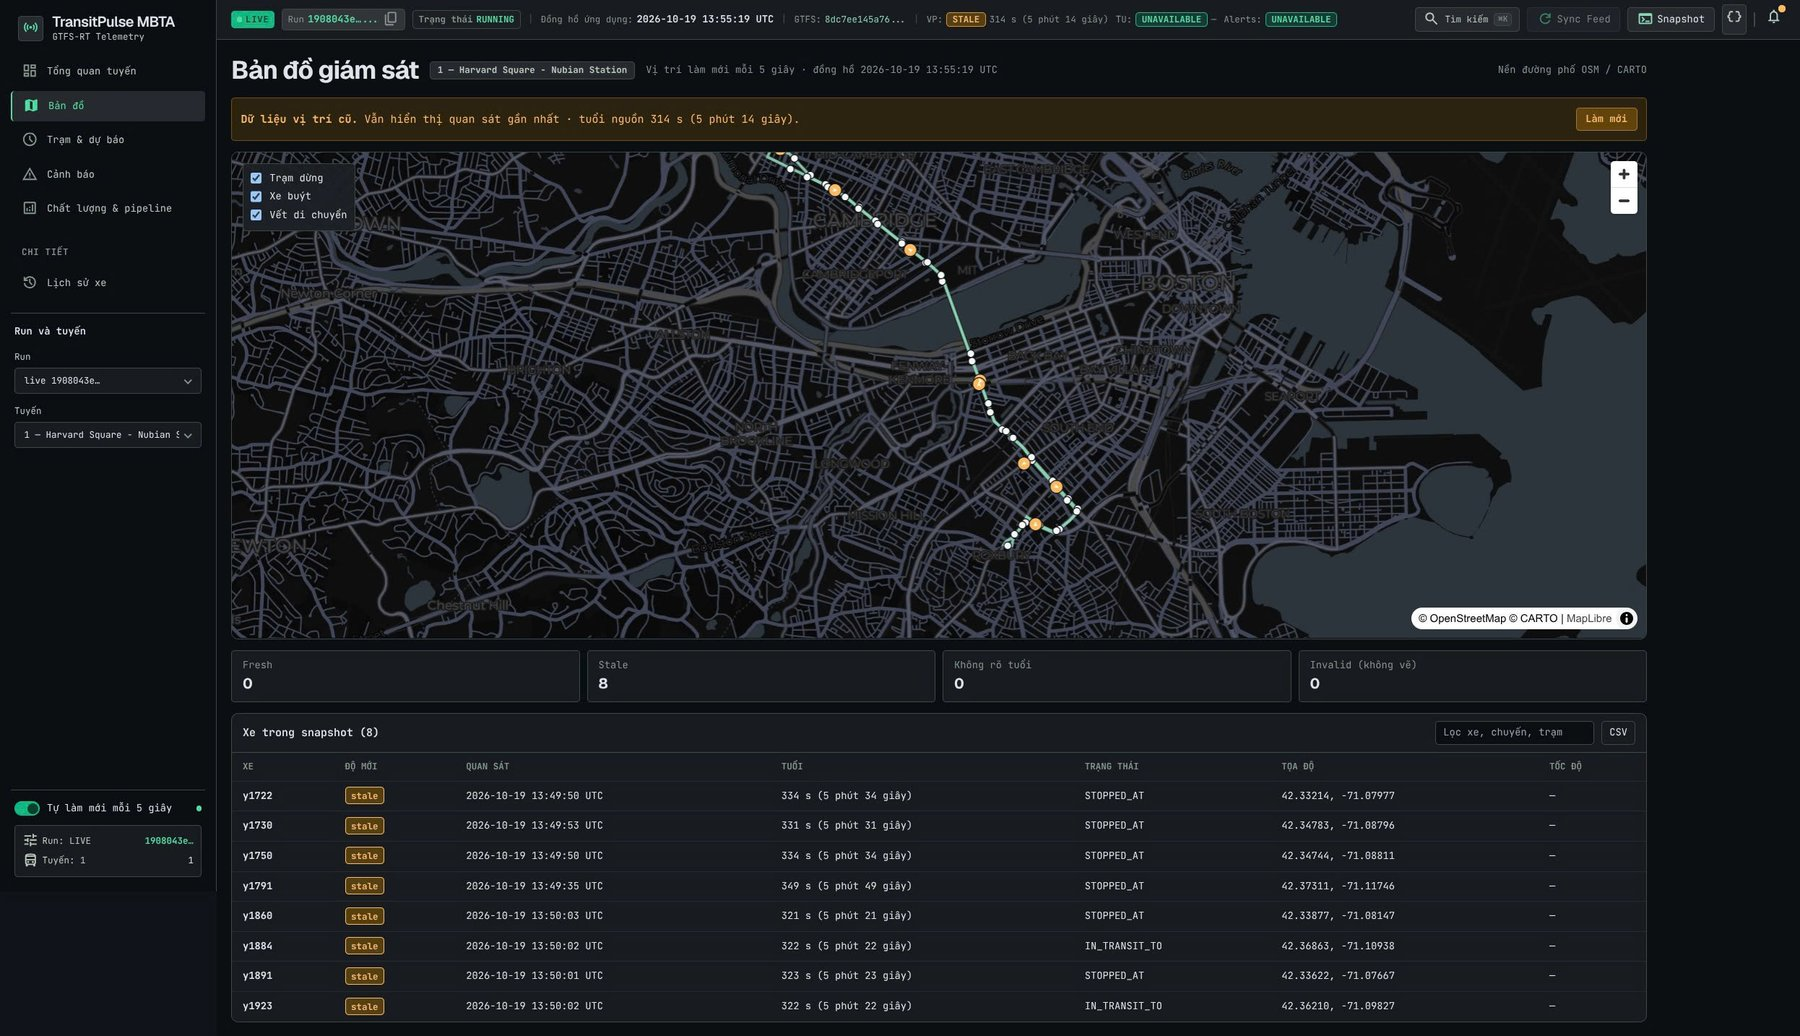
\includegraphics[width=\textwidth]{ui_map.jpg}
\caption{Màn hình Bản đồ hiển thị 8 xe tuyến 1 trên nền CARTO/OpenStreetMap. Cả 8 xe đều ở trạng thái stale, với tuổi dữ liệu 321--349 s so với ngưỡng 120 s. Giao diện giữ vị trí xe và hiển thị thông báo ``Dữ liệu vị trí cũ''.}
\label{fig:ui-map}
\end{figure}

\begin{figure}[H]
\centering
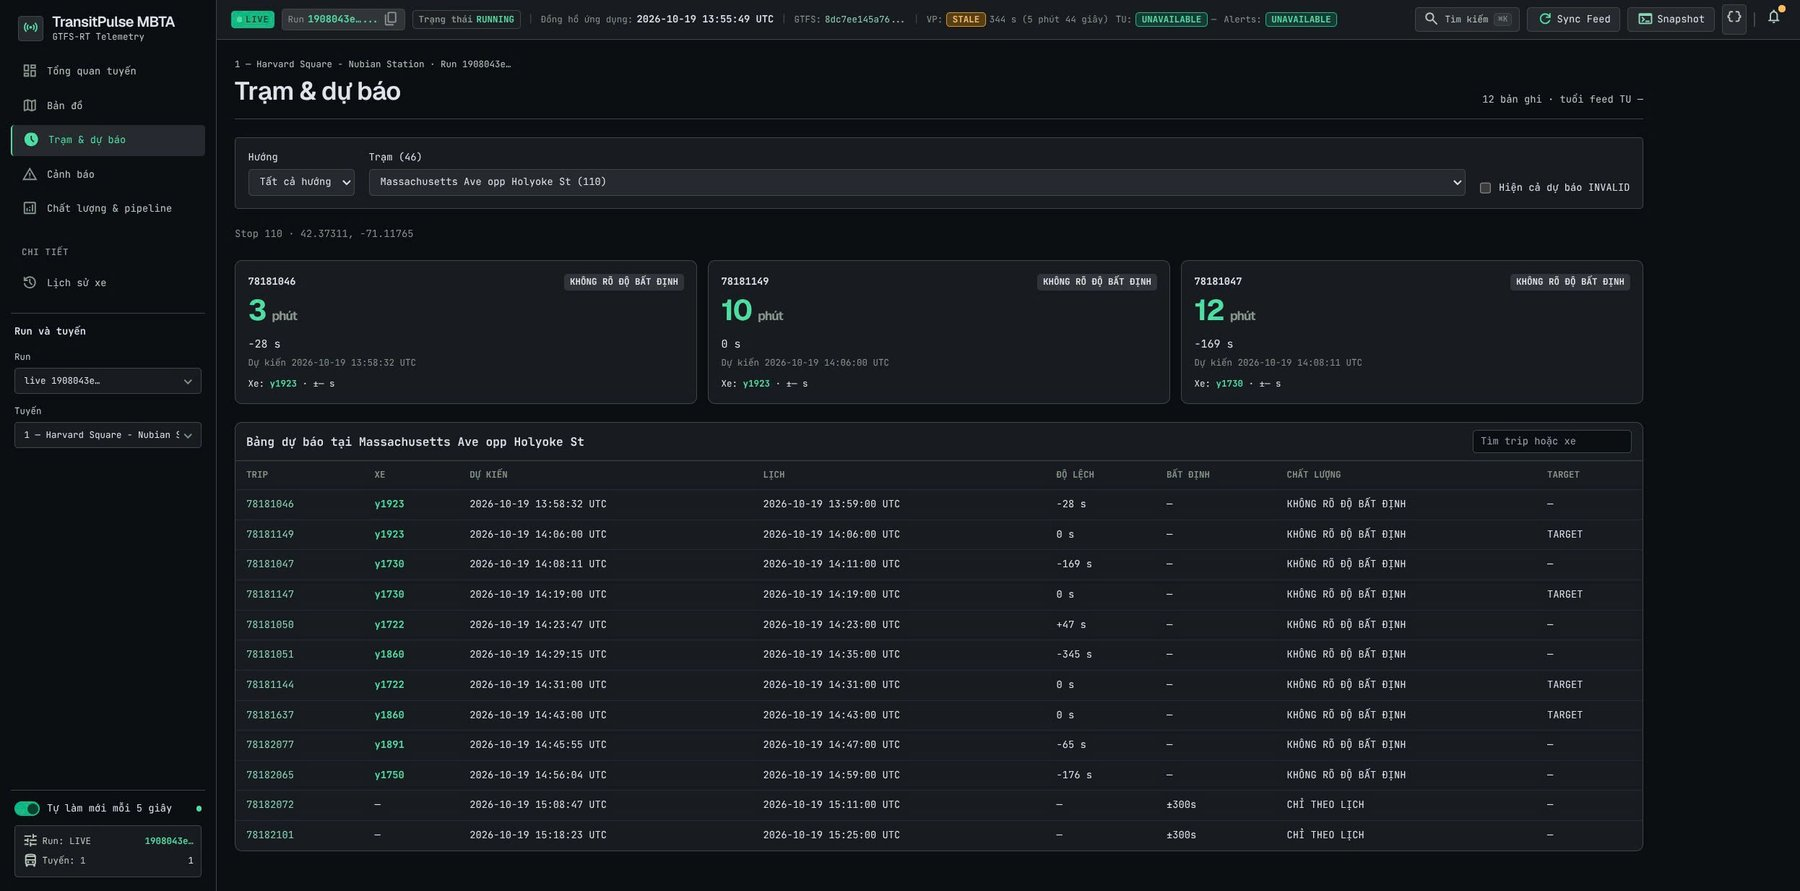
\includegraphics[width=\textwidth]{ui_stops.jpg}
\caption{Màn hình Trạm \& dự báo tại trạm 110 (Massachusetts Ave opp Holyoke St) hiển thị giờ dự kiến, giờ theo lịch, độ lệch có thể âm, nhãn chất lượng và cờ TARGET của từng chuyến. Hai dòng cuối là dự báo chỉ dựa trên lịch, với uncertainty bằng 300.}
\label{fig:ui-stops}
\end{figure}

\begin{figure}[H]
\centering
\begin{subfigure}{\textwidth}
\centering
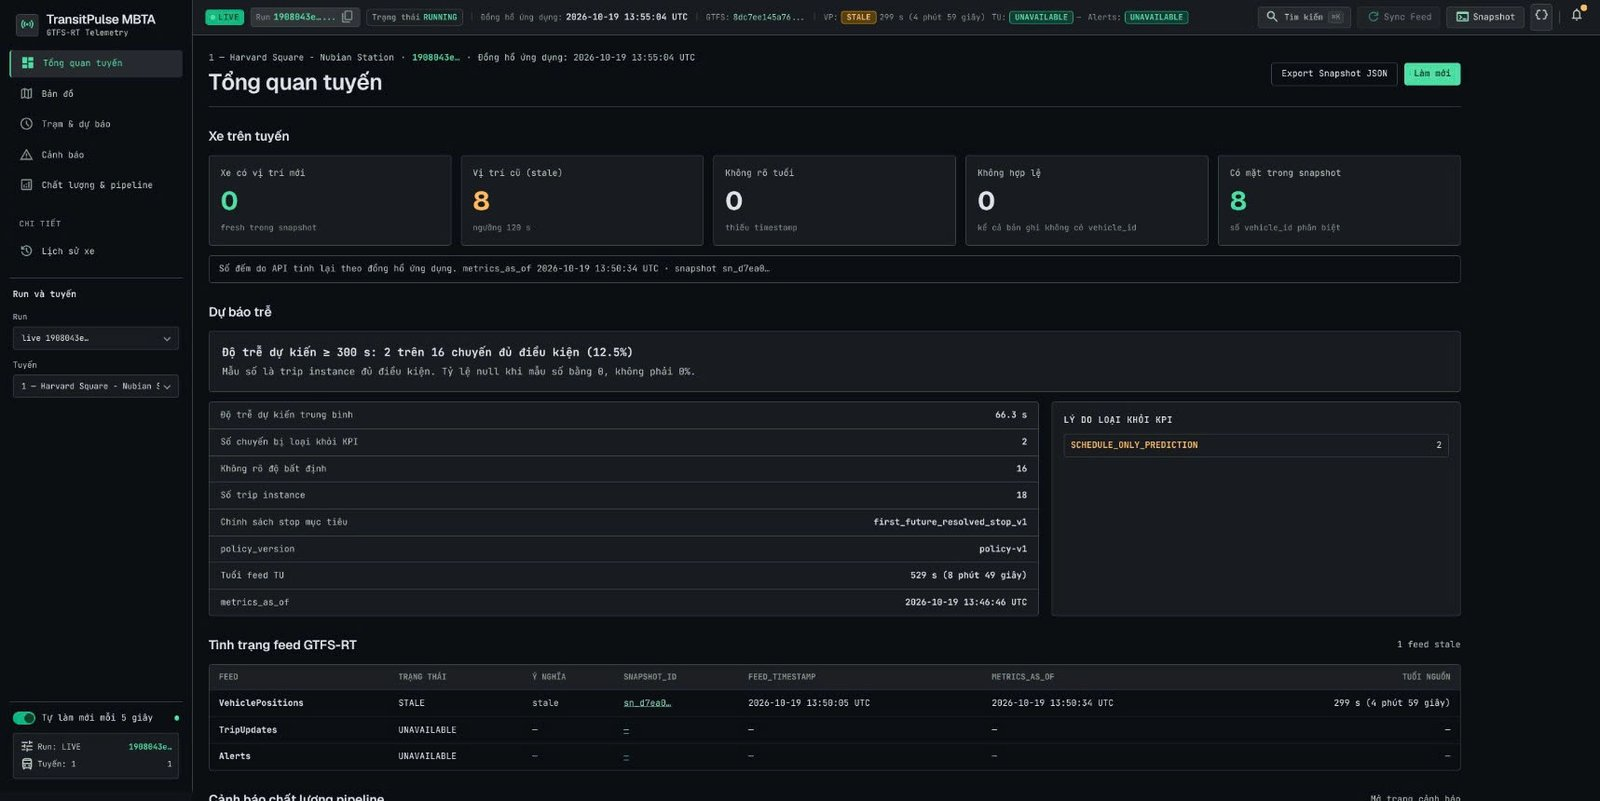
\includegraphics[width=\textwidth]{ui_overview.jpg}
\caption{Màn hình Tổng quan tuyến hiển thị số xe theo mức độ mới, KPI độ trễ dự kiến kèm mẫu số và lý do loại trừ, cùng trạng thái của từng feed.}
\end{subfigure}

\vspace{4mm}
\begin{subfigure}{\textwidth}
\centering
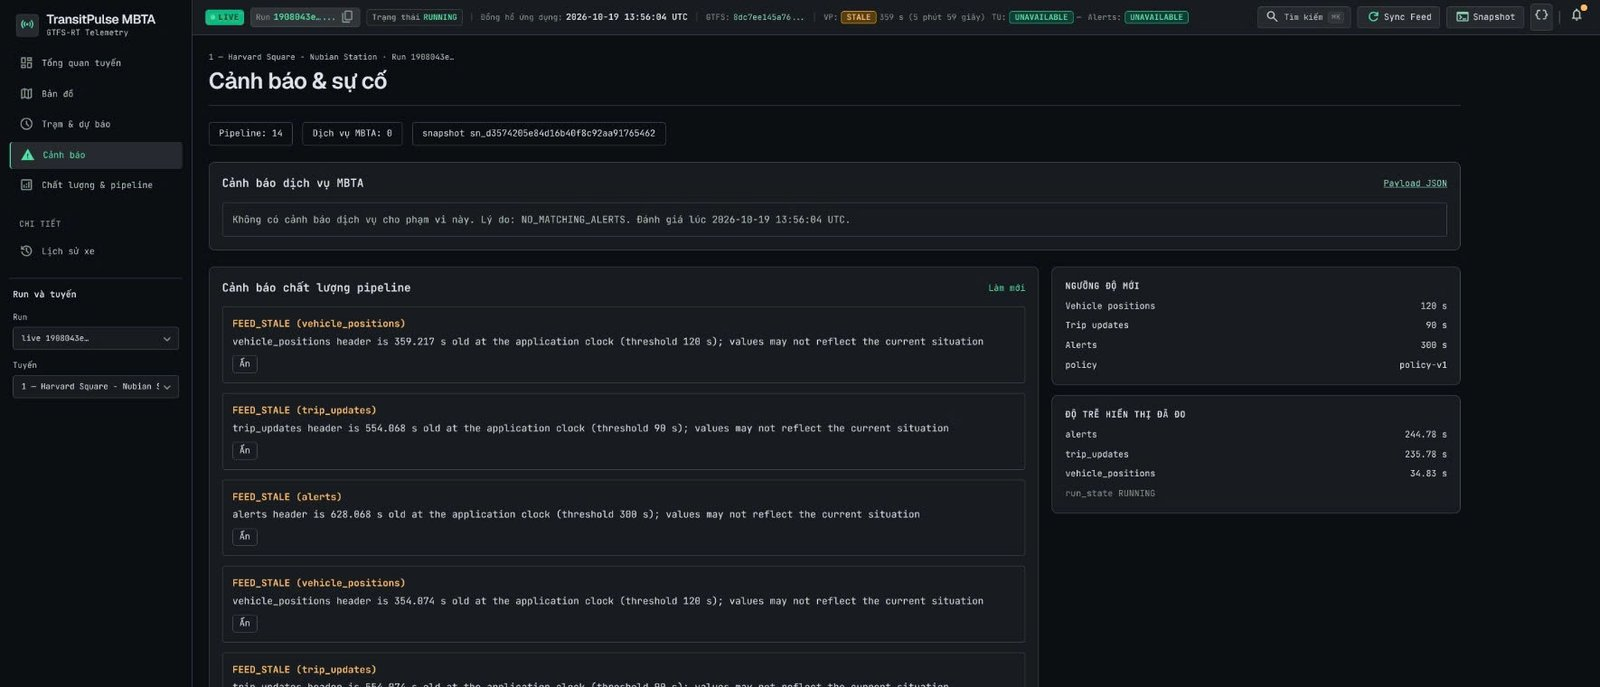
\includegraphics[width=\textwidth]{ui_alerts.jpg}
\caption{Màn hình Cảnh báo trình bày riêng cảnh báo dịch vụ MBTA và cảnh báo chất lượng pipeline. Khung bên phải hiển thị visibility latency gần nhất của từng feed.}
\end{subfigure}
\caption{Màn hình Tổng quan và Cảnh báo trên giao diện React; ảnh đã cắt phần dưới.}
\label{fig:ui-overview}
\end{figure}

Từ các ảnh chụp, có thể ghi nhận thêm bốn điểm trên dữ liệu thực tế:
\begin{itemize}
    \item \textbf{Số lượng chuyến dùng để tính KPI khớp.} Tuyến 1 có 18 trip instance, trong đó 16 chuyến đủ điều kiện và 2 chuyến bị loại với lý do \texttt{SCHEDULE\_ONLY\_PREDICTION}. Các số đếm thỏa mãn $\text{trip\_instances} = \text{eligible} + \sum\text{excluded}$. Có 2/16 chuyến có độ trễ dự kiến từ 300 s trở lên, tương ứng 12,5\%; độ trễ dự kiến trung bình là 66,3 s. Cả 16 chuyến đủ điều kiện đều thiếu trường uncertainty, phù hợp với nhận định rằng dữ liệu xe buýt MBTA thường không có trường này.
    \item \textbf{Độ trễ của từng feed.} Endpoint \ident{/pipeline/status} ghi nhận visibility latency gần nhất là 34,83 s cho VP, 235,78 s cho TU và 244,78 s cho Alerts. Giá trị VP khớp với số liệu lineage 34\,825 ms. Hai generation VP và TU có cùng \ident{metrics_as_of} 13:46:46 và cùng thuộc micro-batch 2. Thứ tự VP $<$ TU $<$ Alerts, cùng chênh lệch khoảng 200 s giữa VP và TU, cho thấy nhánh TU chiếm phần lớn thời gian xử lý của micro-batch.
    \item \textbf{Đánh giá độ mới khi pipeline xử lý chậm.} Lúc 13:55, generation VP hiện hành có \ident{metrics_as_of} 13:50:34, dù bộ thu thập vẫn lấy dữ liệu mỗi 30 s. Trong khoảng 5 phút, bộ xử lý chưa công bố thêm generation VP nào. Khi nhận request, API tính lại tuổi dữ liệu và giao diện chuyển cả 8 xe sang stale, kèm cảnh báo \texttt{FEED\_STALE}. Cơ chế đánh giá độ mới hoạt động đúng thiết kế. Tuy nhiên, việc dữ liệu trở nên cũ cũng cho thấy bộ xử lý không theo kịp tốc độ thu thập, phù hợp với kết quả benchmark ở Mục~\ref{sec:bench}.
    \item \textbf{Lỗi hiển thị còn tồn tại.} Danh sách cảnh báo chất lượng pipeline lặp lại nhiều mục \texttt{FEED\_STALE}, tổng cộng 14 mục cho 3 feed. Ngoài ra, thanh trạng thái phía trên báo TU và Alerts là \texttt{UNAVAILABLE}, trong khi các màn hình vẫn hiển thị KPI từ TU và snapshot cảnh báo hiện hành. Hàm \ident{feedView} trong \ident{frontend/src/format.js} gán trạng thái mặc định \ident{unavailable} nếu response đang dùng không chứa feed tương ứng. Do đó, nguyên nhân nhiều khả năng nằm ở cách hiển thị trạng thái.
\end{itemize}

\subsection{Benchmark}
\label{sec:bench}

\subsubsection{Phương pháp}

Bộ công cụ tại \ident{benchmarks/} đo thông lượng xử lý (throughput), độ trễ (latency), lượng dữ liệu chờ xử lý (backlog), mức sử dụng tài nguyên và thời gian phục hồi trên hệ thống native thực tế. Mỗi lần lặp tạo một run mới, khởi động bộ xử lý và chạy giai đoạn làm nóng (warm-up). Sau đó, công cụ đo trong một khoảng thời gian cố định, ngừng phát dữ liệu và chờ xử lý phần còn lại (drain) cho tới khi backlog bằng 0 hoặc hết thời gian chờ. Các kịch bản được liệt kê trong Bảng~\ref{tab:bench}.

\begin{table}[H]
\centering
\tablefont
\caption{Kịch bản benchmark}
\label{tab:bench}
\begin{tabular}{p{4.46cm}p{5.04cm}p{5.63cm}}
\toprule
\textbf{Kịch bản} & \textbf{Đầu vào} & \textbf{Nội dung đo} \\
\midrule
\texttt{replay\_1x|10x|50x} & Bản ghi dữ liệu thu thập trực tiếp & Thông lượng, độ trễ, backlog, tài nguyên \\
\texttt{stress\_100|500|1000} & Dữ liệu tải cao được sinh, 5 tuyến, 80/20 TU/VP & Như trên, ở 100/500/1000 bản ghi chuẩn hóa/s \\
\texttt{recovery\_partial\_write} & Golden + arm file & Mã thoát 86, khởi động lại cùng checkpoint, thời gian về VP2 \\
\texttt{recovery\_after\_cas} & Golden + arm file & Như trên, gây lỗi sau CAS và trước commit \\
\texttt{recovery\_cassandra\_down} & Golden, dừng Cassandra & Batch thất bại, khởi động lại, thời gian trở về generation đúng \\
\texttt{recovery\_collector\_outbox} & Nguồn giả lập, không kết nối được broker, SIGKILL & Thời gian gửi tiếp từ outbox, số bản ghi mất/trùng \\
\bottomrule
\end{tabular}
\end{table}

Đơn vị đo là \textit{bản ghi chuẩn hóa} (normalized candidate record): một entity Vehicle Positions, một sự kiện arrival hoặc departure của Trip Updates, hoặc một selector của cảnh báo. Các chỉ số được tính từ dữ liệu thu được trong lần chạy như sau:
\begin{itemize}
    \item Các phân vị p50/p95/p99 của visibility latency được lấy từ \ident{snapshot_manifest.visibility_latency_ms} cho các generation được đưa vào hàng đợi trong cửa sổ đo. Generation đến muộn, hết hạn hoặc chưa từng được công bố được đếm riêng.
    \item Thời gian xử lý batch được lấy từ \ident{query_progress.jsonl}. Một batch được tính nếu thời gian chạy của nó có phần giao với cửa sổ đo.
    \item Độ trễ ghi Cassandra được lấy từ log của giai đoạn \ident{cassandra_write}, với một mẫu cho mỗi generation.
    \item Độ trễ API được đo bằng 100 lần gọi \ident{/api/v1/vehicles} sau giai đoạn drain, tính theo thời gian xử lý phía server.
    \item CPU và RSS được lấy mẫu bằng psutil mỗi 2 s. Backlog Kafka được lấy mẫu mỗi 5 s, bằng high watermark trừ end offset đã xử lý.
\end{itemize}
Các phân vị được tính bằng \ident{statistics.quantiles(method="inclusive")}. Nếu số mẫu $n<20$, p95 được ghi \ident{null}; nếu $n<100$, p99 được ghi \ident{null}. Báo cáo luôn kèm số mẫu, giá trị nhỏ nhất và giá trị lớn nhất.

Trong lần chạy \ident{bench-20261024T182433Z}, mỗi kịch bản được lặp một lần, với 180 s làm nóng, 180 s đo và tối đa 60 s chờ xử lý backlog. Các kịch bản tải cao bật whole-stage codegen cho bộ xử lý bằng \ident{TP_SPARK_WHOLE_STAGE=true}. Cả bảy kịch bản đã chạy đều có trạng thái \ident{MEASURED}. Kịch bản replay chưa được chạy do chưa có bản ghi dữ liệu MBTA thực tế.

\subsubsection{Kết quả stress}

Ở cả ba mức tải, publisher giữ tốc độ 0,4 snapshot/s, tương ứng một snapshot VP và một snapshot TU mỗi 5 s. Số bản ghi trong mỗi snapshot được tăng theo mức tải. Kết quả được tổng hợp trong Bảng~\ref{tab:stress} và~\ref{tab:stressres}.

\begin{table}[H]
\centering
\tablefont
\caption{Thông lượng và backlog khi tăng tải bằng dữ liệu sinh, không phải lưu lượng MBTA}
\label{tab:stress}
\begin{tabular}{p{6.6cm}p{2.5cm}p{2.5cm}p{2.5cm}}
\toprule
\textbf{Chỉ số} & \texttt{stress\_100} & \texttt{stress\_500} & \texttt{stress\_1000} \\
\midrule
Bản ghi đầu vào khai báo (bản ghi/s) & 100 & 500 & 1\,000 \\
Snapshot đầu vào (snapshot/s) & 0,40 & 0,40 & 0,40 \\
Lưu lượng Kafka (kB/s) & 15,4 & 75,2 & 149,9 \\
Bản ghi đã xử lý (bản ghi/s) & 6,67 & 25,0 & 50,0 \\
Tỉ lệ so với đầu vào & 6,7\% & 5,0\% & 5,0\% \\
Generation READY trong cửa sổ & 12 & 9 & 3 \\
Dòng Cassandra đã ghi & 2\,460 & 9\,045 & 10\,017 \\
Micro-batch hoàn tất trong cửa sổ & 0 & 0 & 0 \\
Backlog tối đa VP / TU / control (message) & 71 / 71 / 429 & 71 / 71 / 428 & 71 / 72 / 430 \\
Xử lý hết backlog trong 60 s & Không & Không & Không \\
\bottomrule
\end{tabular}
\end{table}

\begin{table}[H]
\centering
\tablefont
\caption{Độ trễ và tài nguyên khi tăng tải}
\label{tab:stressres}
\begin{tabular}{p{6.6cm}p{2.5cm}p{2.5cm}p{2.5cm}}
\toprule
\textbf{Chỉ số} & \texttt{stress\_100} & \texttt{stress\_500} & \texttt{stress\_1000} \\
\midrule
Visibility latency (số mẫu) & -- (0) & -- (0) & -- (0) \\
Ghi Cassandra mỗi generation, p50 (số mẫu) & 0,74 s (12) & 0,89 s (9) & 1,80 s (3) \\
Ghi Cassandra, min -- max & 0,66 -- 0,85 s & 0,85 -- 1,04 s & 1,05 -- 1,80 s \\
API \texttt{/vehicles} p50 / p95 / p99 (ms) & 12,7 / 15,0 / 16,6 & 13,9 / 16,6 / 66,2 & 20,0 / 25,3 / 70,3 \\
CPU bộ xử lý, trung bình / tối đa (\% một lõi) & 159 / 273 & 154 / 286 & 217 / 644 \\
CPU Cassandra / Kafka trung bình (\% một lõi) & 6,7 / 2,7 & 5,5 / 2,4 & 4,7 / 2,3 \\
RSS bộ xử lý tối đa (GiB) & 10,1 & 17,9 & 18,0 \\
Tổng RSS tối đa (GiB) & 15,0 & 22,8 & 23,0 \\
\bottomrule
\end{tabular}
\end{table}

\paragraph{Khả năng theo kịp đầu vào.} Ở cả ba mức tải, bộ xử lý chỉ xử lý được 5--6,7\% số bản ghi đầu vào. Backlog của mỗi topic snapshot tăng đến khoảng 71 thông điệp, gần bằng toàn bộ số snapshot được phát trong cửa sổ đo, và vẫn chưa được xử lý hết sau 60 s drain. Bộ xử lý dành suốt 180 s đo để xử lý một micro-batch dài, không có micro-batch nào hoàn tất nên công cụ không thu được mẫu thời gian batch. Tương tự, không snapshot nào được đưa vào hàng đợi trong cửa sổ đo có thể đọc được trước khi hết giai đoạn drain, nên visibility latency không có mẫu. Với các snapshot này, độ trễ lớn hơn khoảng thời gian từ lúc vào hàng đợi đến cuối giai đoạn drain, tức từ 60 s đến 240 s, cao hơn nhiều so với mục tiêu 10 s. Các generation đạt READY trong cửa sổ đo đều thuộc những snapshot đã vào hàng đợi từ giai đoạn làm nóng.

\paragraph{Thời gian xây dựng generation trên Spark.} Khi chia thời lượng cửa sổ đo cho số generation READY, thời gian tương ứng là khoảng 15 s, 20 s và 60 s mỗi generation. Trong đó, p50 thời gian ghi Cassandra chỉ từ 0,74--1,80 s, chiếm dưới 5\%. Cassandra sử dụng trung bình dưới 7\% một lõi CPU và Kafka dưới 3\%, còn bộ xử lý dùng khoảng 1,5--2,2 lõi, gần hết hai luồng của Spark \ident{local[2]}. Các số liệu này cho thấy nút thắt chủ yếu nằm ở bước xây dựng generation trên Spark cho từng snapshot.

Bộ sinh dữ liệu tải cao phân chia bản ghi theo tỉ lệ 80/20 giữa TU và VP. Với tốc độ mục tiêu $R$, mỗi snapshot VP chứa $R$ bản ghi và mỗi snapshot TU chứa $4R$. Từ số bản ghi đã xử lý và số generation, có thể xác định duy nhất số generation của từng feed:
\begin{itemize}
    \item \ident{stress_100}: 12 generation đều là VP ($12 \times 100 = 1\,200$);
    \item \ident{stress_500}: 9 generation đều là VP ($9 \times 500 = 4\,500$);
    \item \ident{stress_1000}: 1 VP và 2 TU ($1\,000 + 2 \times 4\,000 = 9\,000$). Có 1\,000 bản ghi duy nhất, đúng bằng số quan sát trong một snapshot VP.
\end{itemize}
Như vậy, ở hai mức tải thấp, bộ xử lý chưa hoàn tất generation TU nào trong 180 s đo. Dựa trên hai điểm đo của VP, có thể ước lượng sơ bộ thời gian cho mỗi generation gồm khoảng 14 s chi phí cố định và thêm khoảng 1,25 s cho mỗi 100 bản ghi. Phần chi phí cố định đến từ việc lập kế hoạch và chạy nhiều Spark job cho từng snapshot, lớn hơn đáng kể so với phần tăng theo lượng dữ liệu. Kết hợp với quan sát ở phiên live, trong đó TU chậm hơn VP khoảng 200 s trong cùng micro-batch, nhánh TU là phần tốn thời gian xử lý nhất của pipeline.

\paragraph{Thời gian phản hồi API.} Khi bộ xử lý bão hòa, endpoint \ident{/vehicles} vẫn có p50 trong khoảng 13--20 ms và p95 trong khoảng 15--25 ms. Mỗi request đọc con trỏ hiện hành rồi truy vấn một số phân vùng có giới hạn. Generation bất biến giúp tách việc đọc khỏi quá trình ghi. Ở hai mức tải cao, p99 tăng đến khoảng 66--70 ms. Do chỉ có 100 mẫu, p99 gần với giá trị lớn nhất và dễ thay đổi khi xuất hiện một vài request chậm.

\paragraph{Mức sử dụng bộ nhớ.} RSS của bộ xử lý đạt tối đa 18 GiB, gồm heap driver 16 GiB, Python worker và bộ nhớ ngoài heap. Tổng RSS của hệ thống khoảng 23 GiB, nằm trong ngân sách bộ nhớ của profile \ident{colab-native}.

\subsubsection{Kết quả phục hồi}

Trong mỗi kịch bản, bộ công cụ chủ động gây một lỗi trên tiến trình do nó quản lý khi đang chạy golden fixture. Thời gian phục hồi được tính từ lúc bắt đầu khởi động lại Cassandra hoặc bộ xử lý đến khi generation VP2 trở thành hiện hành và khớp \ident{expected.json}. Riêng với outbox, thời gian được tính từ lúc khởi động lại bộ thu thập đến khi broker xác nhận toàn bộ bản ghi đang chờ gửi. Cột ``Chờ'' thể hiện khoảng thời gian từ lúc gây lỗi đến lúc công cụ phát hiện lỗi và bắt đầu phục hồi; khoảng này được tính riêng.

\begin{table}[H]
\centering
\tablefont
\caption{Kết quả bốn kịch bản phục hồi (một lần lặp mỗi kịch bản)}
\label{tab:recoverybench}
\begin{tabular}{p{3.4cm}p{2.8cm}p{1.45cm}p{1.0cm}p{1.4cm}p{0.95cm}p{1.3cm}}
\toprule
\textbf{Kịch bản} & \textbf{Lỗi được tạo} & \textbf{Mã thoát} & \textbf{Chờ} & \textbf{Phục hồi} & \textbf{Khớp} & \textbf{Mất / trùng} \\
\midrule
\ident{recovery_partial_write} & Dừng sau khi ghi một phần & 86 & 26,8 s & \textbf{43,5 s} & Có & 0 / 0 \\
\ident{recovery_after_cas} & Dừng sau CAS, trước commit & 86 & 25,3 s & \textbf{15,4 s} & Có & 0 / 0 \\
\ident{recovery_cassandra_down} & Dừng Cassandra & 1 & 11,0 s & \textbf{49,5 s} & Có & 0 / 0 \\
\ident{recovery_collector_outbox} & SIGKILL bộ thu thập, không kết nối được broker & SIGKILL & 2,0 s & \textbf{1,0 s} & Có & 0 / 0 \\
\bottomrule
\end{tabular}
\end{table}

Cả bốn kịch bản đều khớp kết quả kỳ vọng, với số bản ghi mất và trùng đều bằng 0. Kết quả này kiểm chứng hoạt động của giao thức công bố generation ở Mục~\ref{sec:publish} và cơ chế outbox qua toàn bộ hệ thống:
\begin{itemize}
    \item \textbf{Dừng đột ngột sau CAS}: thời gian phục hồi là 15,4 s, nhanh nhất trong các kịch bản phục hồi bộ xử lý. Khi Spark xử lý lại micro-batch, manifest đã ở trạng thái READY và con trỏ đã trỏ đúng snapshot. Vì vậy, lần xử lý lại được ghi nhận thành công mà không làm thay đổi kết quả.
    \item \textbf{Dừng đột ngột sau khi ghi một phần}: hệ thống mất 43,5 s để xây dựng và ghi lại generation theo các tham số đã cố định, sau đó mới đánh dấu READY. Trong thời gian này, API tiếp tục đọc generation cũ.
    \item \textbf{Cassandra ngừng hoạt động}: thời gian phục hồi 49,5 s bao gồm cả việc khởi động lại Cassandra. Để đối chiếu, Cassandra mất 42,6 s để khởi động trong lần dựng hạ tầng ở Bảng~\ref{tab:bootstrap}.
    \item \textbf{Outbox}: bộ thu thập bị SIGKILL khi vẫn còn bản ghi chờ gửi. Sau khi khởi động lại, bộ thu thập gửi hết các bản ghi này trong 1,0 s, không ghi nhận bản ghi mất hoặc trùng.
\end{itemize}
Do mỗi kịch bản mới được chạy một lần, các số liệu trên chỉ phản ánh từng lần quan sát và chưa đủ để mô tả phân phối thời gian phục hồi.

Bộ kiểm thử tích hợp IT01--IT16 dưới dạng pytest chưa được chạy trong lần Run All đã ghi nhận, do \ident{RUN_INTEGRATION_TESTS=False}. Các kịch bản phục hồi ở trên kiểm tra cùng nhóm tính chất với IT10--IT12 và việc gửi tiếp từ outbox sau khi khởi động lại, đồng thời đối chiếu với cùng tệp \ident{expected.json}.

\subsection{Tổng hợp mức độ đáp ứng}

Bảng~\ref{tab:status} đối chiếu các yêu cầu với kết quả hiện có và nêu phần còn thiếu. Việc đánh giá phân biệt rõ những nội dung đã được kiểm chứng qua toàn bộ hệ thống, những nội dung mới có kết quả ở mức unit và những kịch bản chưa chạy.

\begingroup\tablefont
\begin{longtable}{p{3.49cm}p{6.40cm}p{5.24cm}}
\caption{Mức độ đáp ứng yêu cầu theo bằng chứng hiện có} \label{tab:status} \\
\toprule
\textbf{Yêu cầu} & \textbf{Bằng chứng end-to-end} & \textbf{Còn thiếu} \\
\midrule
\endfirsthead
\toprule
\textbf{Yêu cầu} & \textbf{Bằng chứng end-to-end} & \textbf{Còn thiếu} \\
\midrule
\endhead
{\tablefont FR01 GTFS tĩnh} & {\tablefont Nạp dữ liệu tĩnh golden và live PASS; 10/10 tuyến hợp lệ} & {\tablefont --} \\
{\tablefont FR02--FR03 Thu thập, Kafka} & {\tablefont Phiên live; truy vết raw $\rightarrow$ Kafka khớp checksum; outbox phục hồi sau SIGKILL, 0 mất, 0 trùng} & {\tablefont IT05, IT13 chưa chạy} \\
{\tablefont FR04--FR07 Xử lý, KPI} & {\tablefont Golden S1--S5 PASS qua API; 940 kiểm thử PASS} & {\tablefont IT06--IT08 chưa chạy} \\
{\tablefont FR08 Cảnh báo} & {\tablefont Golden S1--S5 (alerts) PASS} & {\tablefont IT09 chưa chạy} \\
{\tablefont FR10 Generation, con trỏ} & {\tablefont Golden S3 (trùng), S4 (muộn) PASS; truy vết READY $\rightarrow$ CAS; phục hồi sau ghi một phần, sau CAS và sau khi dừng Cassandra đều khớp kỳ vọng} & {\tablefont IT15 (TTL) chưa chạy} \\
{\tablefont FR11 Replay} & {\tablefont Golden dùng bộ phát lại theo đồng hồ nguồn} & {\tablefont Chưa phát lại bản ghi dữ liệu MBTA thực tế} \\
{\tablefont FR12, NFR05 API, truy vết} & {\tablefont API 200, truy vết nhất quán, giao diện notebook 5 tab, giao diện React qua tunnel (Hình~\ref{fig:ui-map}--\ref{fig:ui-overview})} & {\tablefont Sửa lỗi hiển thị trạng thái feed và cảnh báo lặp; chưa có test UI} \\
{\tablefont NFR02 Phục hồi} & {\tablefont 4/4 kịch bản phục hồi khớp kỳ vọng, 0 mất, 0 trùng; 1,0--49,5 s} & {\tablefont Mới một lần lặp; IT10--IT12 dạng pytest chưa chạy} \\
{\tablefont NFR03 Độ trễ} & {\tablefont \textbf{Chưa đạt.} Live: VP 34,8 s, TU 235,8 s, Alerts 244,8 s; stress: chỉ xử lý 5--6,7\% đầu vào, độ trễ $>$ 60 s} & {\tablefont Tăng thông lượng bộ xử lý; benchmark replay chưa chạy} \\
{\tablefont NFR08 Giới hạn truy vấn} & {\tablefont API \texttt{/vehicles} p95 15--25 ms khi bộ xử lý bão hòa} & {\tablefont --} \\
{\tablefont NFR06 Tái lập} & {\tablefont Checksum của 5 gói phần mềm khớp; đã tạo \texttt{uv.lock}} & {\tablefont Commit tệp \texttt{uv.lock}} \\
\bottomrule
\end{longtable}
\endgroup

\section{Kết luận}
\label{sec:conclusion}

\subsection{Tổng kết}

Báo cáo đã trình bày quá trình xây dựng TransitPulse MBTA, từ thu thập và xử lý đến cung cấp dữ liệu xe buýt MBTA theo thời gian thực bằng Kafka, Spark Structured Streaming và Cassandra. Trọng tâm của đồ án là duy trì kết quả nhất quán khi dữ liệu nguồn có lỗi, sự kiện có thể được nhận nhiều lần và các thành phần không có giao dịch chung. Các kết quả chính gồm:

\begin{itemize}
    \item \textbf{Cơ chế công bố generation}: dữ liệu của mỗi generation được giữ bất biến, còn các tham số trong manifest được cố định từ lần tạo đầu tiên. Hệ thống kiểm tra số dòng trước khi chuyển sang READY và cập nhật con trỏ bằng compare-and-set theo thứ tự dữ liệu nguồn. Cơ chế này giúp API tránh đọc dữ liệu ghi dở, giữ KPI không tăng do bản ghi trùng và ngăn snapshot cũ thay thế trạng thái mới. Trong lần chạy thực tế, khoảng thời gian từ READY đến khi con trỏ được cập nhật bằng CAS là 13 ms.
    \item \textbf{Mô hình lưu trữ theo nhu cầu truy vấn}: Cassandra sử dụng 17 bảng, không cần \ident{ALLOW FILTERING} hay counter. Các bảng phục vụ truy vấn được phân vùng theo \ident{snapshot_id} và tự xóa dữ liệu khi hết TTL.
    \item \textbf{Cách tính chỉ số rõ ràng}: độ mới của dữ liệu được tính lại khi API trả kết quả; giờ GTFS được chuyển đổi có xét ngày đổi giờ mùa hè; mỗi chuyến chỉ đóng góp một sự kiện mục tiêu vào KPI. Tử số và mẫu số được công bố kèm kết quả. Khi mẫu số bằng 0, kết quả KPI nhận giá trị \ident{null} thay vì 0\%.
    \item \textbf{Kết quả kiểm chứng trên Google Colab}: bước khởi tạo kiểm tra checksum của 5 thành phần tải về; 940 kiểm thử đơn vị, môi trường chạy và Spark đều đạt (PASS). Kiểm thử golden smoke từ đầu đến cuối đạt cả 5 bước, bao gồm dữ liệu trùng, dữ liệu đến muộn và tăng đồng hồ nghiệp vụ. Phiên chạy trực tiếp trên 10 tuyến MBTA cũng cho phép truy vết nhất quán từ API về checksum của dữ liệu gốc.
    \item \textbf{Khả năng phục hồi khi có lỗi}: cả bốn kịch bản đo phục hồi đều cho kết quả như kỳ vọng, không mất hoặc trùng bản ghi, với thời gian từ 1,0--49,5 s. Các kịch bản gồm dừng đột ngột sau khi ghi một phần dữ liệu, dừng sau CAS, Cassandra ngừng hoạt động và bộ thu thập bị dừng khi outbox còn bản ghi chờ gửi.
    \item \textbf{Thời gian phản hồi của API}: trong các phép đo, p95 duy trì ở mức 15--25 ms ngay cả khi bộ xử lý bão hòa. Kết quả này gắn với cách đọc dữ liệu theo phân vùng có giới hạn và sử dụng generation bất biến để tách quá trình đọc khỏi quá trình ghi.
\end{itemize}

\subsection{Hạn chế}

\paragraph{Hạn chế về hiệu năng.} Hạn chế lớn nhất là \textbf{chưa đạt mục tiêu p95 visibility latency $<$ 10 s} trên Colab, tức thời gian chờ để dữ liệu có thể được truy vấn còn cao. Ở cả ba mức tải kiểm thử, bộ xử lý chỉ xử lý được 5--6,7\% lượng bản ghi đầu vào và chưa giải quyết hết dữ liệu tồn đọng. Trong phiên chạy trực tiếp, TU và Alerts cần khoảng 4 phút để có thể được đọc qua API. Dữ liệu VP đã chuyển sang trạng thái cũ (stale) khi micro-batch tiếp theo còn chưa hoàn tất. Kết quả đo cho thấy nút thắt nằm ở chi phí cố định lớn khi Spark tạo kết quả cho từng snapshot, đặc biệt ở nhánh TU; Kafka và Cassandra chưa phải các thành phần giới hạn hiệu năng trong các phép đo này.

\paragraph{Hạn chế về kiểm chứng.}
\begin{itemize}
    \item Các kiểm thử tích hợp IT01--IT16 bằng pytest và phép đo hiệu năng khi phát lại dữ liệu MBTA thực tế chưa được thực hiện. Mỗi kịch bản đo hiệu năng mới chạy một lần, và cấu hình Docker Compose cũng chưa được chạy thử.
    \item Phiên demo và golden smoke sử dụng commit \ident{4d6669e}, trong khi phép đo hiệu năng sử dụng commit \ident{ff49f59}. Tệp \ident{uv.lock} được tạo trên Colab nhưng chưa đưa vào commit, nên phiên bản các thư viện phụ thuộc gián tiếp có thể khác nhau giữa hai lần khởi tạo môi trường.
    \item Ảnh chụp giao diện React cho thấy thanh trạng thái báo \texttt{UNAVAILABLE} chưa đúng đối với feed không có trong phản hồi đang dùng, đồng thời danh sách cảnh báo xử lý còn lặp nội dung. Khi rà soát mã nguồn, nhóm cũng nhận thấy màn hình trạm có thể giữ dữ liệu ETA cũ nếu người dùng tiếp tục xem cùng một trạm; trường hợp này chưa được tái hiện khi chạy.
\end{itemize}

\paragraph{Giới hạn trong phạm vi thiết kế.}
\begin{itemize}
    \item Hệ thống sử dụng một Kafka broker và một Cassandra node với hệ số sao chép RF1. Cấu hình này chưa đáp ứng tính sẵn sàng cao và không chịu được sự cố mất máy chủ.
    \item Hệ thống bảo đảm giao nhận at-least-once, kết hợp ghi và công bố dữ liệu theo cách idempotent. Chưa có bảo đảm exactly-once xuyên suốt Kafka, Parquet và Cassandra. Con trỏ điều khiển việc công bố riêng cho từng feed, nên ba feed chưa được cập nhật trong một giao dịch nguyên tử chung.
    \item Thời hạn lưu dữ liệu TTL được tính theo đồng hồ hệ thống và vẫn tiếp tục khi quá trình phát lại đang tạm dừng.
    \item ETA được lấy từ MBTA. Dự án chưa có mô hình ETA riêng và chưa đánh giá độ chính xác do thiếu dữ liệu đối chứng. Dữ liệu xe buýt MBTA thường thiếu trường uncertainty; trong phiên chạy trực tiếp trên tuyến 1, cả 16/16 chuyến đủ điều kiện tính KPI đều thiếu trường này.
    \item Môi trường Colab hoạt động theo phiên, nên máy ảo có thể bị thu hồi và dữ liệu trong thư mục làm việc có thể mất khi máy ảo được đặt lại. Liên kết Cloudflare quick tunnel được truy cập công khai và chưa có xác thực.
\end{itemize}

\subsection{Hướng phát triển}

\begin{enumerate}
    \item \textbf{Ưu tiên tăng năng lực xử lý}: gộp các snapshot cùng feed trong một micro-batch để xử lý bằng một lần chạy Spark, qua đó chia sẻ chi phí cố định khoảng 14 s mỗi generation cho nhiều snapshot. Các hướng khác gồm giảm số Spark action trên mỗi snapshot, tách VP và TU thành các truy vấn độc lập để nhánh VP nhẹ hơn không phải chờ nhánh TU, chuẩn bị trước kế hoạch thực thi Spark và đo lại trên máy có nhiều executor.
    \item \textbf{Bổ sung kết quả kiểm chứng}: đo lại khả năng chịu tải sau khi tối ưu, đo hiệu năng khi phát lại bản ghi MBTA thu trực tiếp trong 2 giờ và chạy IT01--IT16. Mỗi kịch bản cần được lặp nhiều lần, đồng thời đưa \ident{uv.lock} vào commit để cố định phiên bản thư viện.
    \item \textbf{Rút ngắn thời gian nạp dữ liệu tĩnh}: ghi \ident{stop_times_by_trip} song song, bất đồng bộ với số tác vụ đồng thời có giới hạn, hoặc sử dụng Spark Cassandra Connector. Chỉ nạp các chuyến thuộc phạm vi theo dõi.
    \item \textbf{Mở rộng hạ tầng}: thử nghiệm Kafka nhiều broker với nhiều partition theo feed, kết hợp Cassandra ba node, RF3 và \ident{LOCAL_QUORUM}. Khả năng đáp ứng tải cần được đo lại trên cấu hình mở rộng.
    \item \textbf{Đánh giá độ chính xác ETA}: đối chiếu dự báo với thời điểm xe thực tế đến trạm, ước lượng từ chuỗi Vehicle Positions, để xây dựng dữ liệu đối chứng gần đúng.
    \item \textbf{Cải thiện an toàn và giao diện}: nâng Spark lên 3.5.8, bảo vệ tunnel bằng Cloudflare Access, sửa trạng thái feed và gộp các cảnh báo trùng trên giao diện React. Bổ sung kiểm thử hành vi cho việc làm mới ETA và hiển thị uncertainty.
\end{enumerate}


\section{Tài liệu tham khảo}

\begin{thebibliography}{00}

\bibitem{mbta_gtfs}

Massachusetts Bay Transportation Authority,
``MBTA GTFS and GTFS Realtime Documentation.''

https://github.com/mbta/gtfs-documentation

\bibitem{gtfs_static}

MobilityData,
``GTFS Schedule Reference.''

https://gtfs.org/documentation/schedule/reference/

\bibitem{gtfs_rt}

MobilityData,
``GTFS Realtime Reference.''

https://gtfs.org/documentation/realtime/reference/

\bibitem{gtfs_rt_bp}

MobilityData,
``GTFS Realtime Best Practices.''

https://gtfs.org/documentation/realtime/realtime-best-practices/

\bibitem{structured_streaming}

M. Armbrust, T. Das, J. Torres, B. Yavuz, S. Zhu, R. Xin, A. Ghodsi, I. Stoica, and M. Zaharia,
``Structured Streaming: A Declarative API for Real-Time Applications in Apache Spark,''
in \textit{Proceedings of the ACM SIGMOD International Conference on Management of Data}, 2018.

\bibitem{spark}

M. Zaharia, R. S. Xin, P. Wendell, T. Das, M. Armbrust, A. Dave, X. Meng, J. Rosen, S. Venkataraman,
M. J. Franklin, A. Ghodsi, J. Gonzalez, S. Shenker, and I. Stoica,
``Apache Spark: A Unified Engine for Big Data Processing,''
\textit{Communications of the ACM}, vol. 59, no. 11, 2016.

\bibitem{kafka}

J. Kreps, N. Narkhede, and J. Rao,
``Kafka: a Distributed Messaging System for Log Processing,''
in \textit{Proceedings of the NetDB Workshop}, 2011.

\bibitem{cassandra}

A. Lakshman and P. Malik,
``Cassandra: A Decentralized Structured Storage System,''
\textit{ACM SIGOPS Operating Systems Review}, vol. 44, no. 2, 2010.

\bibitem{paxos}

L. Lamport,
``Paxos Made Simple,''
\textit{ACM SIGACT News}, vol. 32, no. 4, 2001.

\bibitem{dataflow}

T. Akidau, R. Bradshaw, C. Chambers, S. Chernyak, R. J. Fernández-Moctezuma, R. Lax, S. McVeety, D. Mills,
F. Perry, E. Schmidt, and S. Whittle,
``The Dataflow Model: A Practical Approach to Balancing Correctness, Latency, and Cost in Massive-Scale,
Unbounded, Out-of-Order Data Processing,''
\textit{Proceedings of the VLDB Endowment}, vol. 8, no. 12, 2015.

\bibitem{ddia}

M. Kleppmann,
\textit{Designing Data-Intensive Applications}.
O'Reilly Media, 2017.

\bibitem{microservices_patterns}

C. Richardson,
\textit{Microservices Patterns: With Examples in Java}.
Manning Publications, 2018.

\bibitem{repo}

Mã nguồn TransitPulse MBTA.

https://github.com/nqMinh-GR/de\_btl

\end{thebibliography}

\newpage
%-------------------- main --------------------%
\newpage
\end{document}
